% ===========================================================================
% RELATORIO — Roteiro 2, Amplificador Operacional: Introducao
% ENE0046 Laboratorio de Eletronica 2026/2 — Equipe 1, Turma 04
% ===========================================================================
\documentclass[11pt,a4paper]{article}
\input{estilo-relatorio}

% --------------------------- IDENTIFICACAO ---------------------------------
\roteiro{2}{Amplificador Operacional: Introdução}
\aturma{04}

\autorum{Ana Luísa Reis Nascente}{211045688}
\autordois{Gabriel de Sousa}{211056000}
% ---------------------------------------------------------------------------

\begin{document}
\capa

\begin{resumo}
Este relatório projeta, simula e monta quatro configurações clássicas de amplificador
operacional — seguidor de tensão, amplificador não inversor, somador inversor e amplificador
de diferença — com o LM741 e o TL064. O dimensionamento de cada circuito parte de uma
especificação numérica própria: individual, derivada da matrícula, na etapa de simulação, e
comum à equipe na etapa de bancada, de modo que a montagem física é compartilhada por todos os
integrantes enquanto o projeto simulado é pessoal. Os quatro blocos se comportaram, de modo
geral, como a teoria de realimentação negativa prevê: o seguidor isolou a carga do divisor
resistivo, o não inversor manteve seu ganho ao trocar de AmpOp, e o amplificador de diferença
respondeu à substituição forçada de componente com uma rejeição de modo comum pior que a
prevista. O somador, por sua vez, revelou um problema real de bancada na fonte de um dos
sinais de entrada. O relatório fecha comparando, para cada circuito, o cálculo analítico, a
simulação e a medição, discutindo de onde vem cada divergência encontrada.
\end{resumo}

\section{Introdução}

Um amplificador operacional a malha aberta tem ganho enorme e mal definido — na prática,
inútil sozinho. É a realimentação negativa que o transforma em blocos previsíveis: um
seguidor de tensão que isola um sensor de alta impedância da carga que ele alimenta, um
amplificador que multiplica um sinal pequeno por um fator fixo antes de um conversor, um
somador que combina um sinal com um nível de referência sem que um interfira no outro, e um
amplificador de diferença que extrai um sinal de poucos milivolts em meio a uma interferência
de modo comum muito maior — o mesmo princípio usado para captar um sinal cardíaco sob o ruído
da rede elétrica. Cada um desses quatro blocos aparece dezenas de vezes num equipamento de
instrumentação real, quase sempre em cascata.

Este roteiro investiga os quatro ao mesmo tempo, com o LM741 e o TL064, dimensionando cada um
a partir de uma especificação numérica derivada da matrícula do estudante — de modo que cada
integrante da equipe projeta um conjunto de ganhos diferente, mas todos resolvendo a mesma
estrutura de circuito. A série de resistores é limitada à E12, o que raramente entrega o valor
exato pedido pela álgebra; o quanto essa aproximação afasta o circuito do ideal, e o quanto a
tolerância real do componente (contra o valor nominal impresso) afasta o circuito simulado do
circuito montado, são as duas perguntas que atravessam o relatório inteiro.

A etapa de bancada usa uma segunda especificação, definida pelo número da equipe na turma, não
pela matrícula individual — assim a montagem física é comum a todos os integrantes, enquanto a
simulação de projeto continua sendo individual.

O restante deste relatório está organizado como segue: a Seção~2 deduz as expressões usadas em
cada um dos quatro blocos; a Seção~3 aplica essas expressões à especificação da matrícula e
escolhe os componentes comerciais; a Seção~4 descreve como cada simulação e cada montagem foram
feitas; a Seção~5 traz os resultados numéricos; a Seção~6 discute as divergências entre projeto,
simulação e medição; e a Seção~7 fecha com as conclusões.

\section{Fundamentação teórica}

\subsection{Seguidor de tensão e o efeito de carregamento}

Um divisor resistivo (fonte $V_i$, $R_1$ em série, $R_2$ para o terra) é, do ponto de vista do
nó de saída, um equivalente de Thévenin:

\begin{equation}
V_{th} = V_i \cdot \frac{R_2}{R_1+R_2}, \qquad R_{th} = R_1 \parallel R_2
\label{eq:thevenin}
\end{equation}

Ao ligar uma carga $R_L$ diretamente nesse nó, ela forma um divisor adicional com $R_{th}$, e a
tensão cai:

\begin{equation}
V_{carga} = V_{th}\cdot\frac{R_L}{R_L+R_{th}}, \qquad
\text{queda} = \frac{V_{th}-V_{carga}}{V_{th}} = \frac{R_{th}}{R_L+R_{th}}
\label{eq:queda}
\end{equation}

A queda percentual depende só da razão entre $R_{th}$ e $R_L$, não do valor absoluto de
$V_{th}$ — é esse o critério de projeto do divisor. Um seguidor de tensão (AmpOp com a saída
ligada diretamente à entrada inversora) entre o divisor e a carga resolve o problema porque a
entrada do AmpOp tem impedância altíssima: praticamente nenhuma corrente é drenada do divisor,
que passa a operar como se estivesse em vazio, e a impedância de saída do AmpOp é baixíssima, de
modo que a carga não consegue impor queda nenhuma na saída do seguidor. É o mesmo recurso pelo
qual um multímetro de $10\,\text{M}\Omega$ de entrada mede sem alterar o que mede.

\subsection{Amplificador não inversor}

Com o AmpOp em realimentação negativa e ganho de malha aberta muito grande, as duas entradas
ficam praticamente no mesmo potencial (curto virtual). Como a entrada não inversora recebe
$v_i$ diretamente, o nó inversor também fica em $v_i$. A corrente que entra por $R_g$ (do nó
inversor ao terra) é a mesma que sai por $R_f$ (do nó inversor à saída), já que a entrada do
AmpOp não drena corrente:

\begin{equation}
\frac{v_i}{R_g} = \frac{v_o - v_i}{R_f} \quad\Rightarrow\quad
G = \frac{v_o}{v_i} = 1 + \frac{R_f}{R_g}
\label{eq:naoinversor}
\end{equation}

O ganho depende só da razão $R_f/R_g$, não do AmpOp específico, desde que o ganho de malha
aberta continue muito maior que $G$. A alimentação simétrica limita a excursão de saída: acima
de uma certa amplitude de entrada, $G\cdot v_i$ ultrapassa o que o estágio de saída consegue
entregar, e a saída satura um pouco abaixo da tensão de alimentação.

\subsection{Somador inversor}

Aqui a entrada não inversora vai ao terra, e o curto virtual força o nó inversor também a
$0\,\text{V}$ — um terra virtual. As duas entradas, cada uma com seu resistor, não se enxergam
porque cada uma vê o nó inversor como um curto para o terra, isolado da outra pela realimentação.
Por superposição, a corrente que cada entrada injeta no terra virtual sai inteira pelo resistor
de realimentação $R_f$:

\begin{equation}
\frac{V_1}{R_1}+\frac{V_2}{R_2} = -\frac{V_o}{R_f}
\quad\Rightarrow\quad
V_o = -\left(\frac{R_f}{R_1}V_1+\frac{R_f}{R_2}V_2\right) = -(k_1V_1+k_2V_2)
\label{eq:somador}
\end{equation}

Cada peso $k_i$ é a razão entre $R_f$ e o resistor daquela entrada — quanto menor o resistor de
entrada frente a $R_f$, maior o peso dessa entrada na soma.

\subsection{Amplificador de diferença}

Com quatro resistores e o AmpOp em realimentação negativa, a entrada não inversora vê um
divisor entre $R_3$ e $R_4$ alimentado por $V_{ref}$, e o curto virtual iguala o nó inversor a
esse mesmo potencial:

\begin{equation}
V_+ = V_{ref}\cdot\frac{R_4}{R_3+R_4}
\label{eq:diferenca-vmais}
\end{equation}

Fazendo o balanço de corrente no nó inversor (entrada $v_s$ por $R_1$, realimentação por $R_2$,
igual ao raciocínio do somador) e substituindo $V_-=V_+$, chega-se à expressão geral, válida
mesmo sem casamento entre os dois ramos:

\begin{equation}
V_o = V_{ref}\cdot\frac{R_4}{R_3+R_4}\cdot\frac{R_1+R_2}{R_1} \; - \; v_s\cdot\frac{R_2}{R_1}
\label{eq:diferenca-geral}
\end{equation}

Quando os dois ramos são casados ($R_3=R_1$, $R_4=R_2$), essa expressão se reduz à forma
conhecida $V_o = A_d(V_+-V_-)$ com $A_d=R_2/R_1$, e o ganho de modo comum (a resposta do
circuito a um mesmo sinal aplicado às duas entradas) vai exatamente a zero. Na prática, nenhum
par de resistores é idêntico: usando \eqref{eq:diferenca-geral} com $v_s=V_{ref}$ (mesmo sinal
nas duas entradas), o ganho de modo comum residual é

\begin{equation}
A_{cm} = \left|\frac{R_4}{R_3+R_4}\cdot\frac{R_1+R_2}{R_1} - \frac{R_2}{R_1}\right|
\label{eq:acm}
\end{equation}

e a rejeição de modo comum é $\text{CMRR} = 20\log_{10}(A_d/A_{cm})$, em dB. Mesmo com os quatro
resistores idealmente casados, o AmpOp real ainda tem uma rejeição de modo comum finita, própria
do dispositivo — é essa componente que domina quando o descasamento dos resistores é pequeno.

\section{Especificação e projeto}

\begin{espec}
Matrícula \mat{211045688}, na forma ABCDEFGHI: A=2, B=1, C=1, D=0, EF=45, GH=68, I=8.
\begin{align*}
V_{carga} &= 2+\text{EF}/33 = 2+45/33 = 3{,}364\text{ V} \\
\text{queda mín.} &= 25+\text{GH}/5 = 25+68/5 = 38{,}6\% \\
G &= 4+\left[(7\cdot\text{EF}+3\cdot\text{GH})\bmod 81\right]/10 = 4+33/10 = 7{,}3 \\
k_1 &= 2+(\text{EF}\bmod 4) = 3 \\
k_2 &= 6+(\text{GH}\bmod 4) = 6 \\
A_d &= 2+\left[(3\cdot\text{GH}+7\cdot I)\bmod 90\right]/10 = 10{,}0
\end{align*}
\end{espec}

Resistores da série E12, entre $1\,\text{k}\Omega$ e $82\,\text{k}\Omega$, cada perna da rede de
realimentação com até dois resistores em série. Alimentação simétrica de $\pm15\,\text{V}$.

\subsection{Seguidor de tensão}

A especificação da matrícula fixa dois alvos: a tensão sobre a carga já com o divisor
carregado, e a queda mínima que o divisor deve suportar. O segundo alvo é o que dimensiona o
circuito — impondo-o em \eqref{eq:queda} com $R_L=1\,\text{k}\Omega$ e depois resolvendo o
divisor por \eqref{eq:thevenin} com $V_i=10\,\text{V}$:

\begin{formula}
\begin{align*}
R_{th} &\geq \frac{\text{queda}}{1-\text{queda}}\cdot R_L = 0{,}629\times 1000 \approx 629\,\Omega \\[4pt]
\text{Escolhido: } R_{th}&\approx 666{,}7\,\Omega \text{ (folga confortável)}
\;\Rightarrow\; R_1=1{,}2\,\text{k}\Omega,\;\; R_2=1{,}5\,\text{k}\Omega \text{ (E12)}
\end{align*}
\end{formula}

\begin{center}
\begin{tabular}{@{}lrrr@{}}
\toprule
\textbf{Grandeza} & \textbf{Teórico} & \textbf{Adotado} & \textbf{Desvio} \\
\midrule
$R_{th}$ mínimo & $629\,\Omega$ & $666{,}7\,\Omega$ (folga) & — \\
$V_{carga}$ (com carga) & $3{,}364$~V & $3{,}333$~V & $-0{,}9\%$ \\
Queda & $38{,}6\%$ (mínimo) & $40{,}0\%$ & acima do mínimo \\
\bottomrule
\end{tabular}
\end{center}

\subsection{Amplificador não inversor}

De \eqref{eq:naoinversor}, $R_f/R_g = G-1 = 6{,}3$. Testando combinações E12 (um ou dois
resistores em série por perna), a que menos se afasta é $R_g=8{,}2\,\text{k}\Omega$,
$R_f=47\,\text{k}\Omega+4{,}7\,\text{k}\Omega=51{,}7\,\text{k}\Omega$:

\begin{center}
\begin{tabular}{@{}lrrr@{}}
\toprule
\textbf{Grandeza} & \textbf{Teórico} & \textbf{Adotado} & \textbf{Desvio} \\
\midrule
$R_f/R_g$ & $6{,}300$ & $6{,}30488$ & $+0{,}08\%$ \\
$G$ & $7{,}300$ & $7{,}30488$ & $+0{,}07\%$ \\
\bottomrule
\end{tabular}
\end{center}

Alternativas de resistor único (ex.\ $R_g=1\,\text{k}\Omega$, $R_f=6{,}8\,\text{k}\Omega$) davam
desvio de até $6{,}8\%$; o par com dois resistores em série reduziu o erro em duas ordens de
grandeza.

\subsection{Somador inversor}

De \eqref{eq:somador}, $R_f/R_1=k_1=3$ e $R_f/R_2=k_2=6$. Com
$R_f=22\,\text{k}\Omega$, $R_1=5{,}6\,\text{k}\Omega+1{,}8\,\text{k}\Omega=7{,}4\,\text{k}\Omega$
e $R_2=2{,}7\,\text{k}\Omega+1\,\text{k}\Omega=3{,}7\,\text{k}\Omega$:

\begin{center}
\begin{tabular}{@{}lrrr@{}}
\toprule
\textbf{Grandeza} & \textbf{Teórico} & \textbf{Adotado} & \textbf{Desvio} \\
\midrule
$k_1$ & $3{,}000$ & $2{,}973$ & $-0{,}90\%$ \\
$k_2$ & $6{,}000$ & $5{,}946$ & $-0{,}90\%$ \\
\bottomrule
\end{tabular}
\end{center}

Com $V_1=V_2=0{,}5\,\text{V}$ (dentro da faixa $0{,}1$–$1\,\text{V}$ pedida), a saída projetada
fica em $V_o=-(2{,}973\times0{,}5+5{,}946\times0{,}5)=-4{,}46\,\text{V}$, com folga de
${\approx}9{,}5\,\text{V}$ até a saturação (${\gg}2\,\text{V}$ pedidos).

\subsection{Amplificador de diferença}

De \eqref{eq:diferenca-vmais}--\eqref{eq:acm} com ramos casados, $R_2/R_1=A_d=10{,}0$. A razão
$10{,}0$ é exata entre dois valores E12 consecutivos de década:

\begin{center}
\begin{tabular}{@{}lrrr@{}}
\toprule
\textbf{Grandeza} & \textbf{Teórico} & \textbf{Adotado} & \textbf{Desvio} \\
\midrule
$R_1=R_3$ & — & $1\,\text{k}\Omega$ & — \\
$R_2=R_4$ & — & $10\,\text{k}\Omega$ & — \\
$A_d$ & $10{,}000$ & $10{,}000$ & $0{,}00\%$ \\
\bottomrule
\end{tabular}
\end{center}

Foi o único item do roteiro em que a razão E12 bateu exatamente com o pedido, sem precisar de
resistores em série.

\section{Metodologia}

Cada AmpOp foi trazido para o LTspice como um símbolo de cinco terminais construído a partir do
subcircuito em \texttt{ene0046.lib} (\texttt{item\_6.asy} para o LM741, \texttt{item\_7.asy}
para o TL064), com a ordem de pinos conferida diretamente no cabeçalho de cada subcircuito do
arquivo — as duas peças não compartilham a mesma ordem de terminais. Cada simulação individual
usa alimentação $\pm15\,\text{V}$ empilhada (duas fontes de 15\,V com o terra no nó do meio),
técnica mais confiável do que ajustar a polaridade de duas fontes independentes na mão.

\subsection{Simulação de projeto, uma por integrante}

\subsubsection*{Ana Luísa Reis Nascente — matrícula 211045688}

Os cinco itens da especificação individual foram simulados em arquivos separados
(\texttt{item\_1.asc} a \texttt{item\_5.asc}), cada um com uma única diretiva de análise ativa:

\begin{itemize}
\item \textbf{item\_1} — seguidor de tensão, ponto de operação (\texttt{.op}) nas três
  condições (divisor em vazio, com carga ligada diretamente, e com o seguidor entre o divisor e
  a carga), lado a lado no mesmo esquemático.
\item \textbf{item\_2} — não inversor, transiente (\texttt{.tran}) com varredura paramétrica
  (\texttt{.step}) da amplitude de entrada em duas condições: uma linear e outra levando a
  saída à saturação.
\item \textbf{item\_3} e \textbf{item\_4} — somador inversor, o mesmo circuito em ponto de
  operação (\texttt{.op}, com $V_1{=}V_2{=}0{,}5\,\text{V}$) e em varredura DC
  (\texttt{.dc}, $V_1$ de 0 a 1\,V com $V_2$ fixo).
\item \textbf{item\_5} — amplificador de diferença com o TL064, transiente com as duas condições
  de ensaio (diferencial e modo comum) em circuitos separados dentro do mesmo arquivo.
\end{itemize}

\begin{figure}[htb]
\centering
% \includegraphics[width=0.8\linewidth]{item_1_circuito.png}
\fbox{\parbox[c][3.2cm][c]{0.8\linewidth}{\centering\color{cinza}
  substitua por \texttt{\textbackslash includegraphics\{item\_1\_circuito.png\}}}}
\caption{Esquemático do item\_1 (seguidor de tensão): as três condições de operação lado a
lado no mesmo ponto de operação.}
\label{fig:item1}
\end{figure}

\subsubsection*{Gabriel de Sousa — matrícula 211056000}

Matrícula 211056000, na forma ABCDEFGHI: A=2, B=1, C=1, D=0, EF=56, GH=00, I=0.
\begin{align*}
V_{carga} &= 2+\text{EF}/33 = 2+56/33 = 3{,}697\text{ V} \\
\text{queda mín.} &= 25+\text{GH}/5 = 25+0/5 = 25{,}0\% \\
G &= 4+\left[(7\cdot\text{EF}+3\cdot\text{GH})\bmod 81\right]/10 = 4+68/10 = 10{,}8 \\
k_1 &= 2+(\text{EF}\bmod 4) = 2 \\
k_2 &= 6+(\text{GH}\bmod 4) = 6 \\
A_d &= 2+\left[(3\cdot\text{GH}+7\cdot I)\bmod 90\right]/10 = 2{,}0
\end{align*}

Os cinco itens foram simulados nos mesmos arquivos individuais (\texttt{item\_1.asc} a
\texttt{item\_5.asc}, na pasta \texttt{Simulacoes}), seguindo a mesma estrutura de
esquemático usada por Ana Luísa:

\begin{itemize}
\item \textbf{item\_1} — seguidor de tensão, ponto de operação (\texttt{.op}) nas três
  condições (divisor em vazio, com $R_L=1\,\text{k}\Omega$ ligada diretamente, e com o
  seguidor LM741 entre o divisor e a carga), lado a lado no mesmo esquemático. Divisor
  $R_1{=}1{,}2\,\text{k}\Omega$, $R_2{=}2{,}2\,\text{k}\Omega$ ($R_{th}{\approx}776{,}5\,
  \Omega$), $V_i{=}10\,\text{V}$.
\item \textbf{item\_2} — não inversor, transiente (\texttt{.tran}) com \texttt{.step} da
  amplitude de entrada em duas condições ($A{=}1\,\text{V}$ e $A{=}1{,}5\,\text{V}$).
  $R_g{=}2\,\text{k}\Omega$, $R_f{=}18\,\text{k}\Omega+1\,\text{k}\Omega=19\,\text{k}
  \Omega$, dando $G=1+19/2=10{,}5$.
\item \textbf{item\_3} e \textbf{item\_4} — somador inversor, o mesmo circuito em ponto de
  operação (\texttt{.op}, com $V_1{=}V_2{=}0{,}5\,\text{V}$) e em varredura DC
  (\texttt{.dc}, $V_1$ de 0 a 1\,V com $V_2{=}0{,}5\,\text{V}$ fixo). $R_1{=}3{,}3\,\text{k}
  \Omega+2{,}7\,\text{k}\Omega=6\,\text{k}\Omega$, $R_2{=}1\,\text{k}\Omega+1\,\text{k}
  \Omega=2\,\text{k}\Omega$, $R_f{=}12\,\text{k}\Omega$, dando $k_1{=}12/6{=}2{,}0$ e
  $k_2{=}12/2{=}6{,}0$ — casamento exato com a especificação, sem erro de arredondamento E12.
\item \textbf{item\_5} — amplificador de diferença com o TL064, transiente com os dois
  ensaios (diferencial e modo comum) em circuitos separados no mesmo arquivo. Todos os
  quatro resistores em $1{,}5\,\text{k}\Omega$/$12\,\text{k}\Omega$, dando $A_d{=}12/1{,}5{=}
  8{,}0$ — valor que \textbf{não} bate com o $A_d{=}2{,}0$ calculado acima da especificação
  (a razão adotada no esquemático é a mesma do somador, $12\,\text{k}\Omega/1{,}5\,\text{k}
  \Omega$; ainda falta conferir se houve troca do valor-alvo ao montar este item — ver
  nota na Seção~5.1).
\end{itemize}

\begin{figure}[htb]
\centering
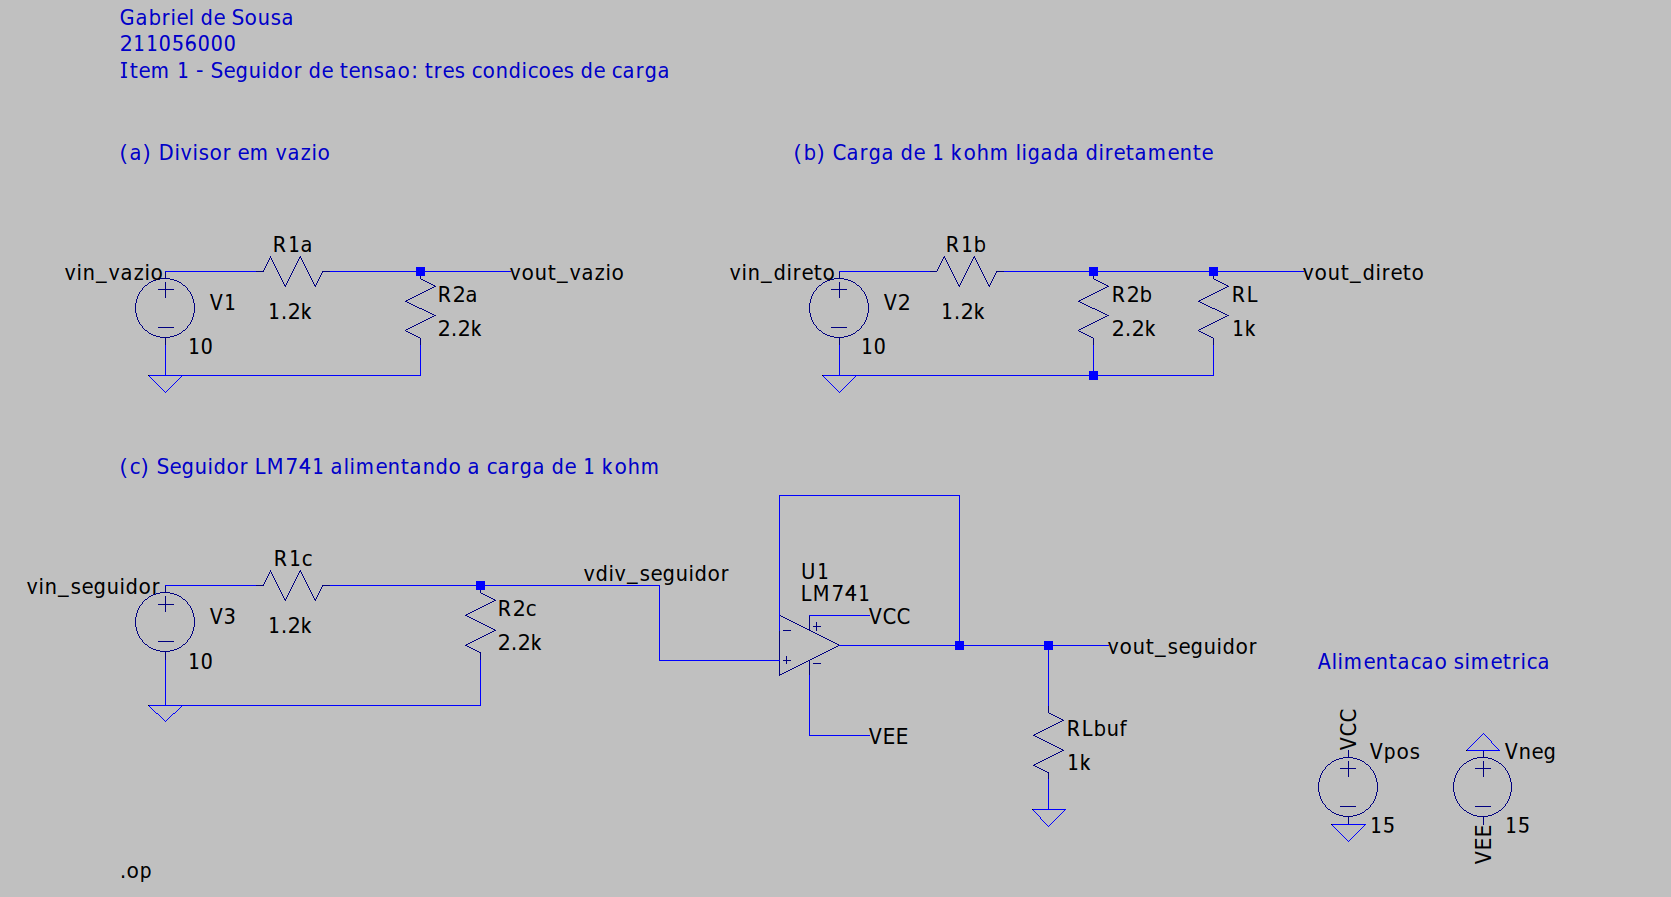
\includegraphics[width=0.95\linewidth]{item_1_gabriel.png}
\caption{Esquemático do item\_1 de Gabriel (seguidor de tensão): as três condições de
operação lado a lado no mesmo ponto de operação.}
\label{fig:item1-gabriel}
\end{figure}

\begin{figure}[htb]
\centering
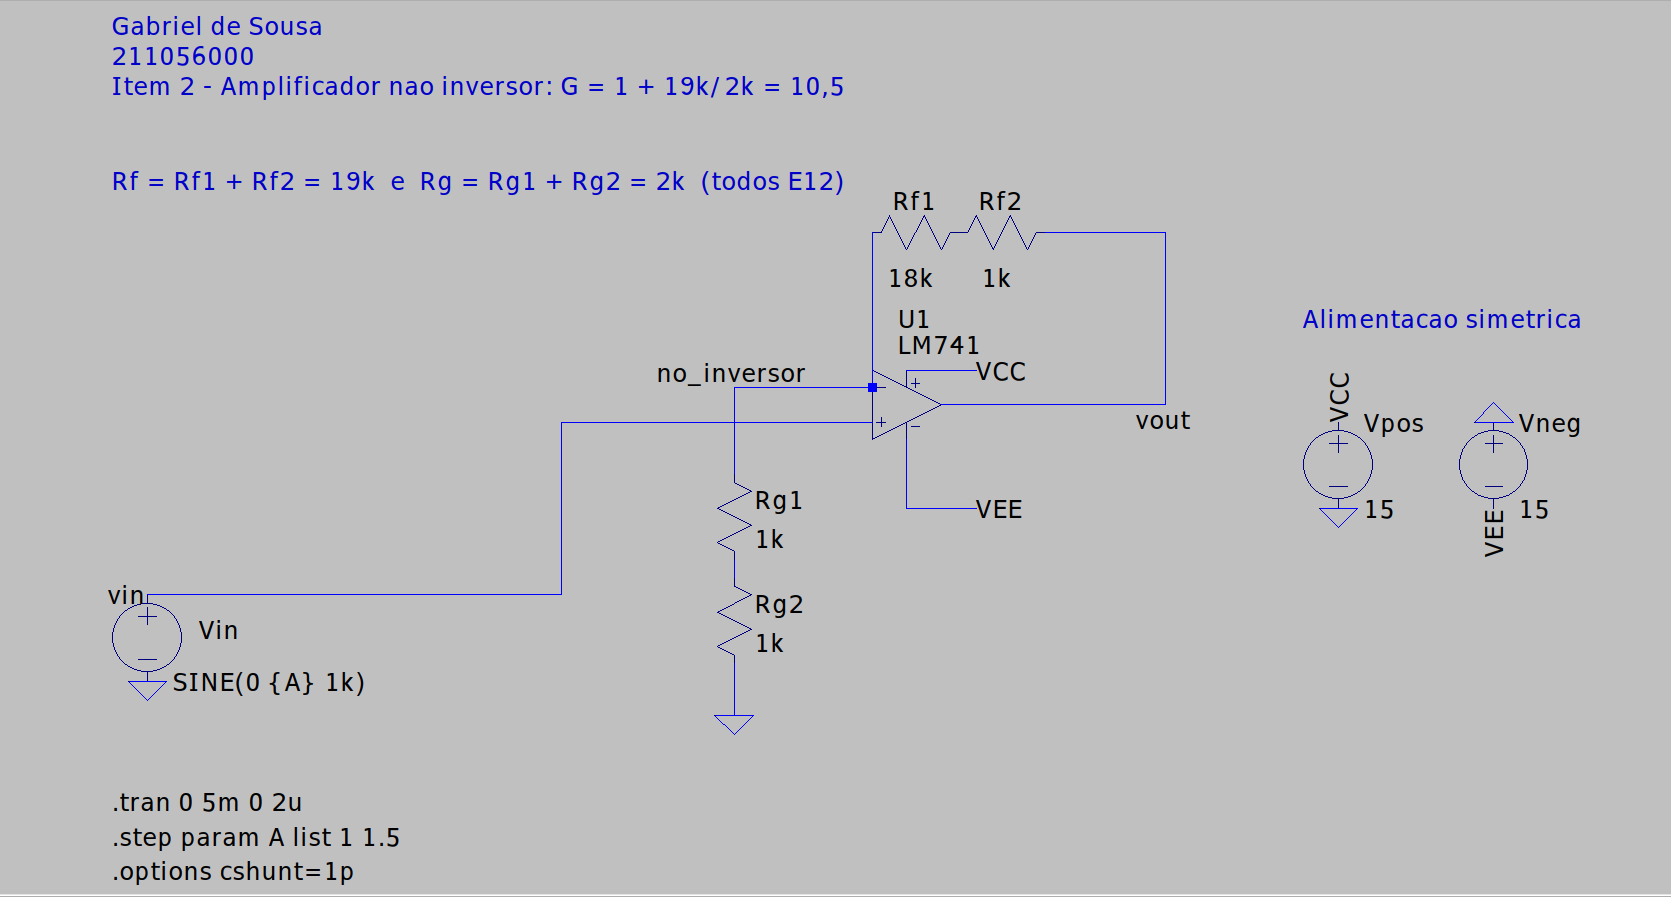
\includegraphics[width=0.85\linewidth]{item_2_gabriel.png}
\caption{Esquemático do item\_2 de Gabriel (não inversor): varredura da amplitude de
entrada por \texttt{.step}.}
\label{fig:item2-gabriel}
\end{figure}

\begin{figure}[htb]
\centering
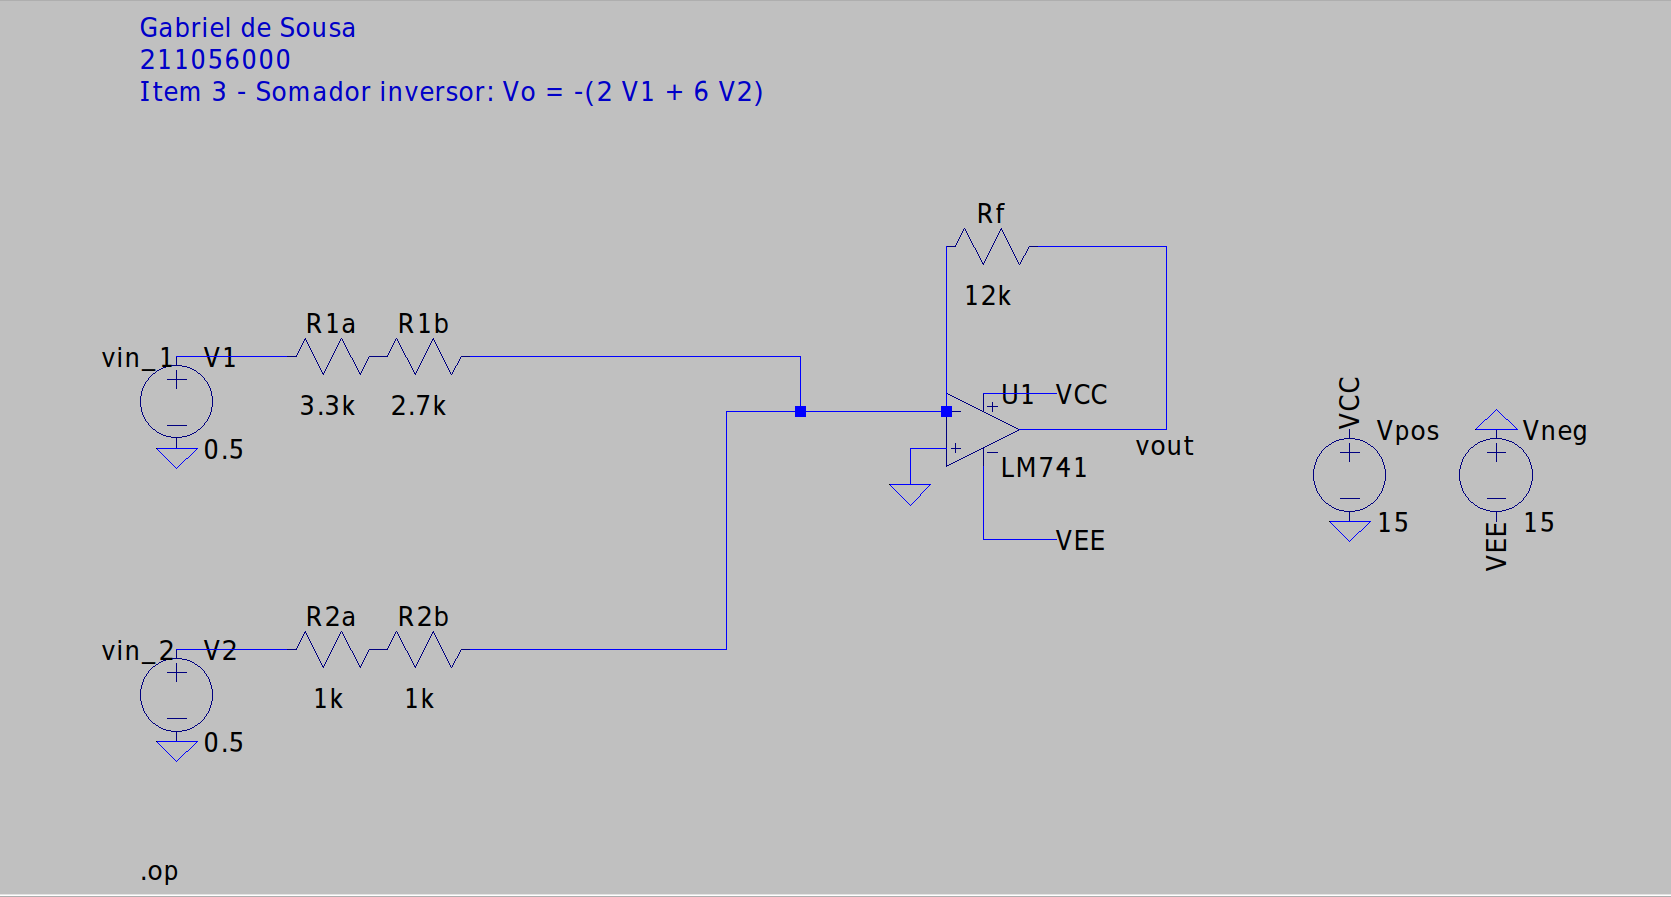
\includegraphics[width=0.85\linewidth]{item_3_gabriel.png}
\caption{Esquemático do item\_3 de Gabriel (somador inversor, ponto de operação).}
\label{fig:item3-gabriel}
\end{figure}

\begin{figure}[htb]
\centering
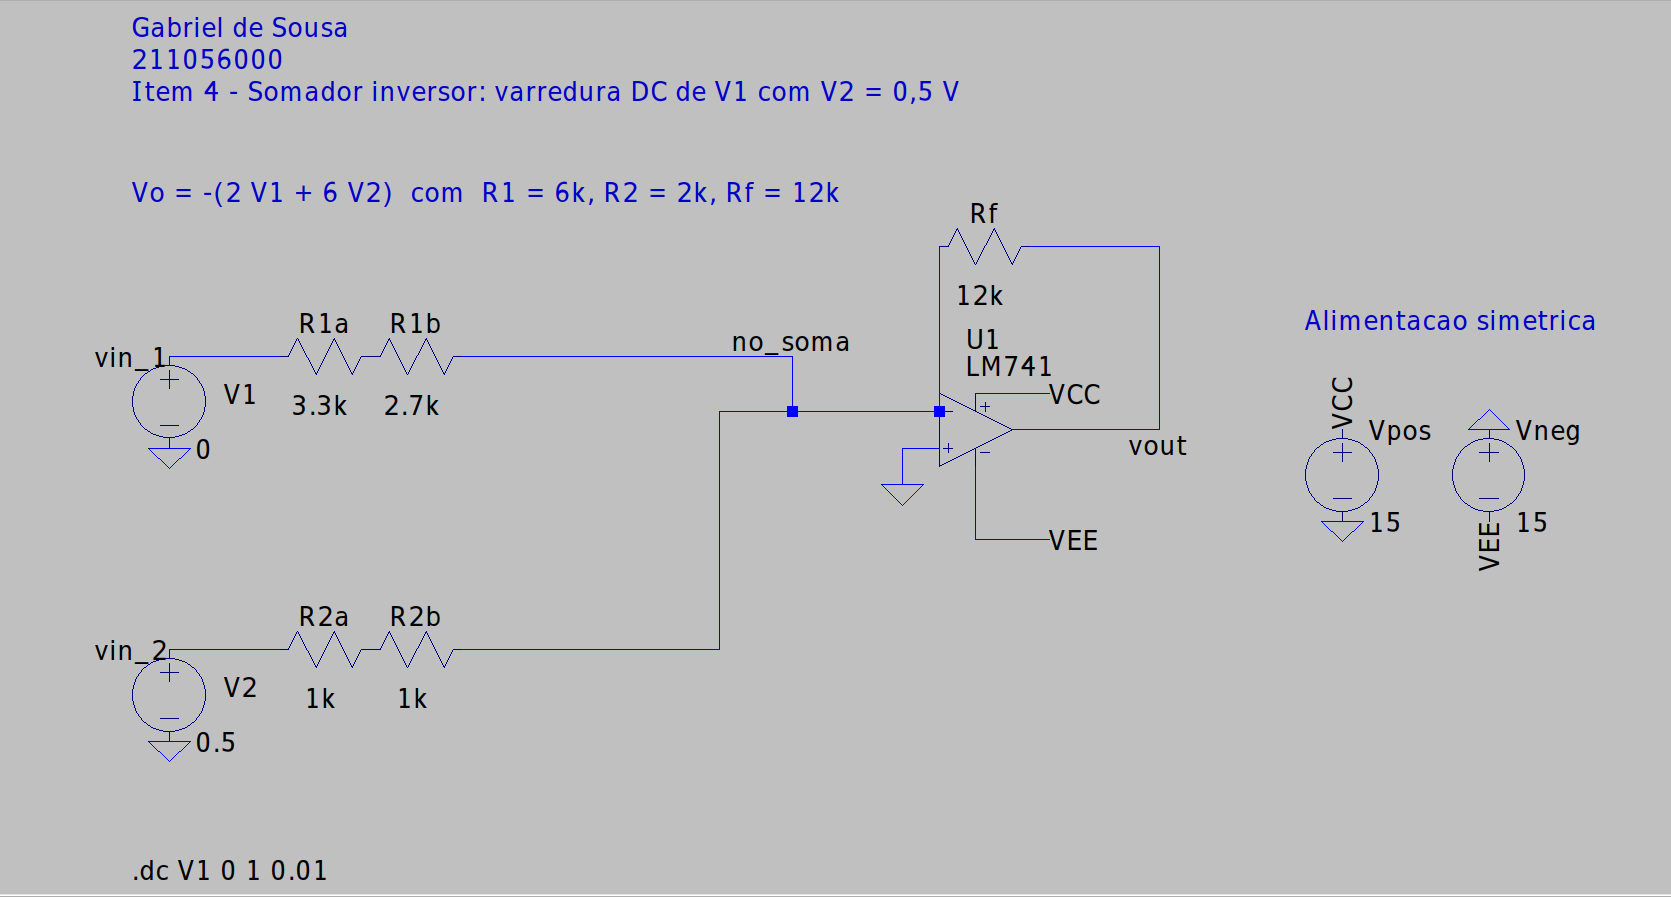
\includegraphics[width=0.85\linewidth]{item_4_gabriel.png}
\caption{Esquemático do item\_4 de Gabriel (somador inversor, varredura DC de $V_1$).}
\label{fig:item4-gabriel}
\end{figure}

\begin{figure}[htb]
\centering
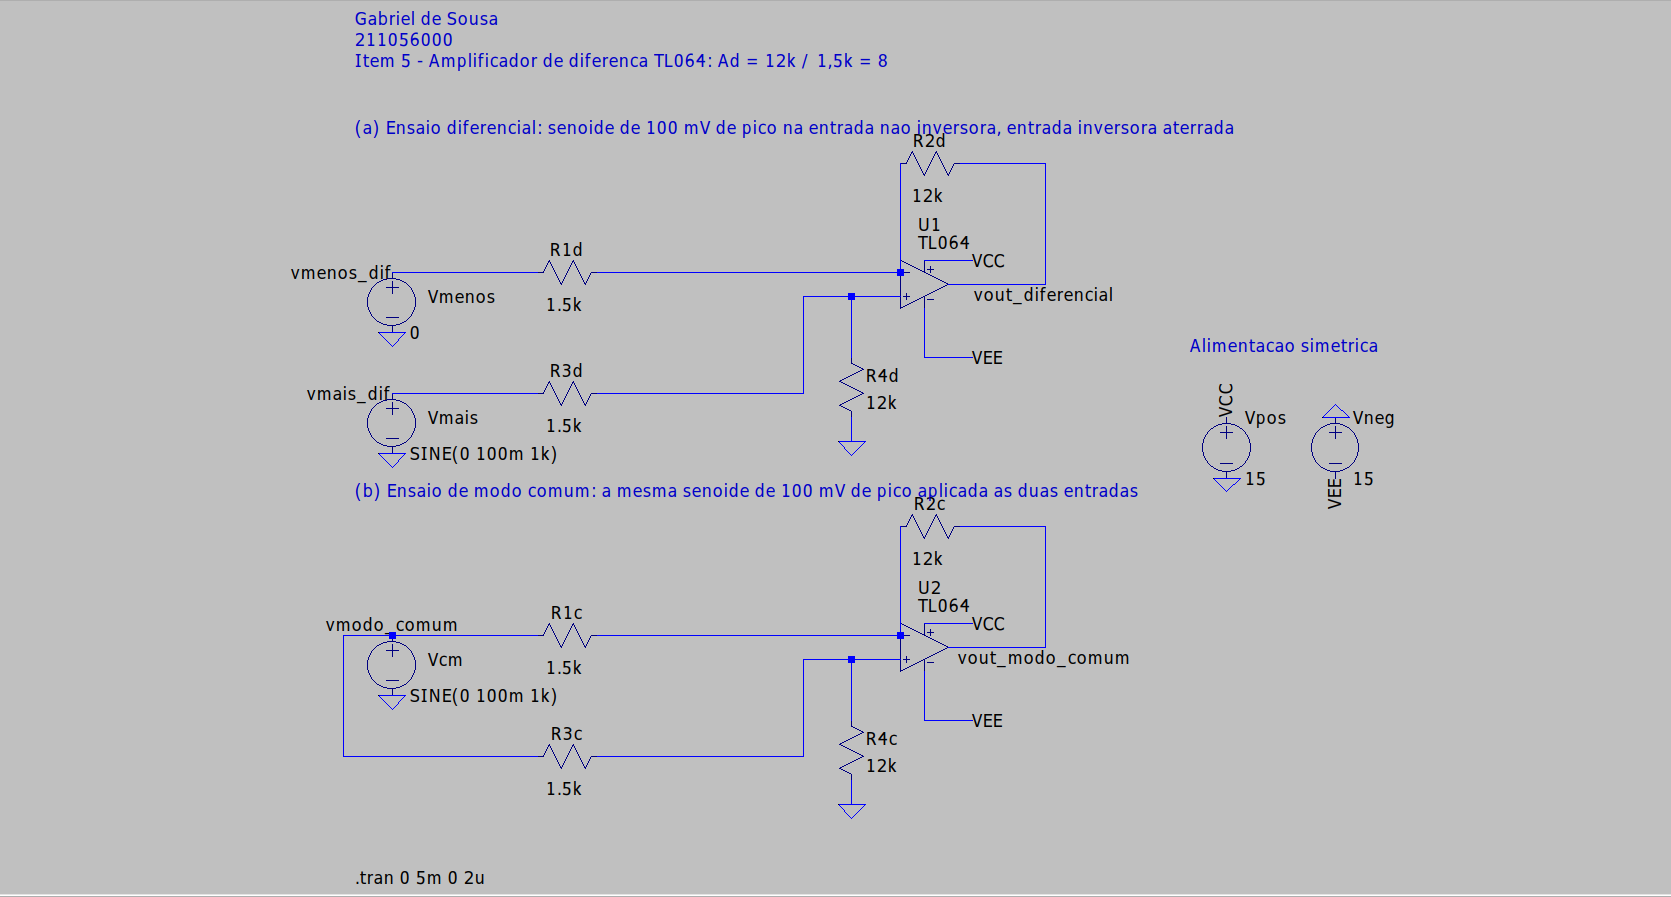
\includegraphics[width=0.95\linewidth]{item_5_gabriel.png}
\caption{Esquemático do item\_5 de Gabriel (amplificador de diferença, TL064): ensaios
diferencial e de modo comum lado a lado.}
\label{fig:item5-gabriel}
\end{figure}

\subsection{Montagem em bancada}

A especificação de bancada é definida pelo número da equipe na turma (Equipe~1), independente
da matrícula de qualquer integrante:
$\text{queda}=29\%$, $G_v=2{,}00$, $k_1{=}1{,}00$ e $k_2{=}1{,}22$, $V_1{=}4{,}0\,\text{V}$ e
$V_2{=}-4{,}0\,\text{V}$, $A_d=1{,}50$. A série E12 disponível na bancada vai de
$820\,\Omega$ a $33\,\text{k}\Omega$, com no máximo um resistor por perna (sem combinações em
série, diferente da etapa de simulação).

Componentes escolhidos, na série E12 disponível na bancada:

\begin{center}
\begin{tabular}{@{}llr@{}}
\toprule
\textbf{Circuito} & \textbf{Componente} & \textbf{Nominal} \\
\midrule
Seguidor & $R_1=R_2$ & $820\,\Omega$ \\
Seguidor & $R_L$ & $1\,\text{k}\Omega$ \\
Não inversor & $R_g=R_f$ & $10\,\text{k}\Omega$ \\
Somador & $R_1{=}R_f$ & $2{,}2\,\text{k}\Omega$ \\
Somador & $R_2$ & $1{,}8\,\text{k}\Omega$ \\
Diferença & $R_1{=}R_3$ & $10\,\text{k}\Omega$ \\
Diferença & $R_2{=}R_4$ & $15\,\text{k}\Omega$ \\
\bottomrule
\end{tabular}
\end{center}

Só os quatro resistores do amplificador de diferença foram pesados individualmente no
multímetro antes da montagem ($R_1{=}9{,}97\,\text{k}\Omega$, $R_2{=}14{,}95\,\text{k}\Omega$,
$R_3{=}10{,}05\,\text{k}\Omega$, $R_4{=}15{,}01\,\text{k}\Omega$ — usados na Seção~5.4); os
demais componentes foram conferidos só pelo código de cores.

O amplificador de diferença foi montado com o \textbf{LM741} em vez do TL064 especificado pelo
roteiro: o encapsulamento TL064/TL074 não estava disponível na bancada no momento da montagem.
A topologia é idêntica — só muda a numeração dos pinos usados (o LM741 é um único AmpOp por
encapsulamento, mas os dois ensaios, diferencial e de modo comum, já eram feitos sem desmontar
o circuito, então um único AmpOp basta).

Os capacitores de desacoplamento de $100\,\text{nF}$ entre cada alimentação e o terra, previstos
no roteiro, não foram usados nessa montagem por orientação verbal do professor em aula.

Cada circuito foi montado, medido e desmontado na ordem: alimentação e conferência dos
$\pm15\,\text{V}$ nos pinos do encapsulamento antes de qualquer sinal; seguidor (quatro
condições); não inversor (duas amplitudes, mais a troca de LM741 por um AmpOp livre do TL064
sem alterar $R_f/R_g$, e a medida da tensão de alimentação real para comparar com a saturação);
somador (com $V_2$ ajustado na fonte antes de ligar ao circuito); e por fim o amplificador de
diferença, com os dois ensaios feitos sem desmontar.

\begin{figure}[htb]
\centering
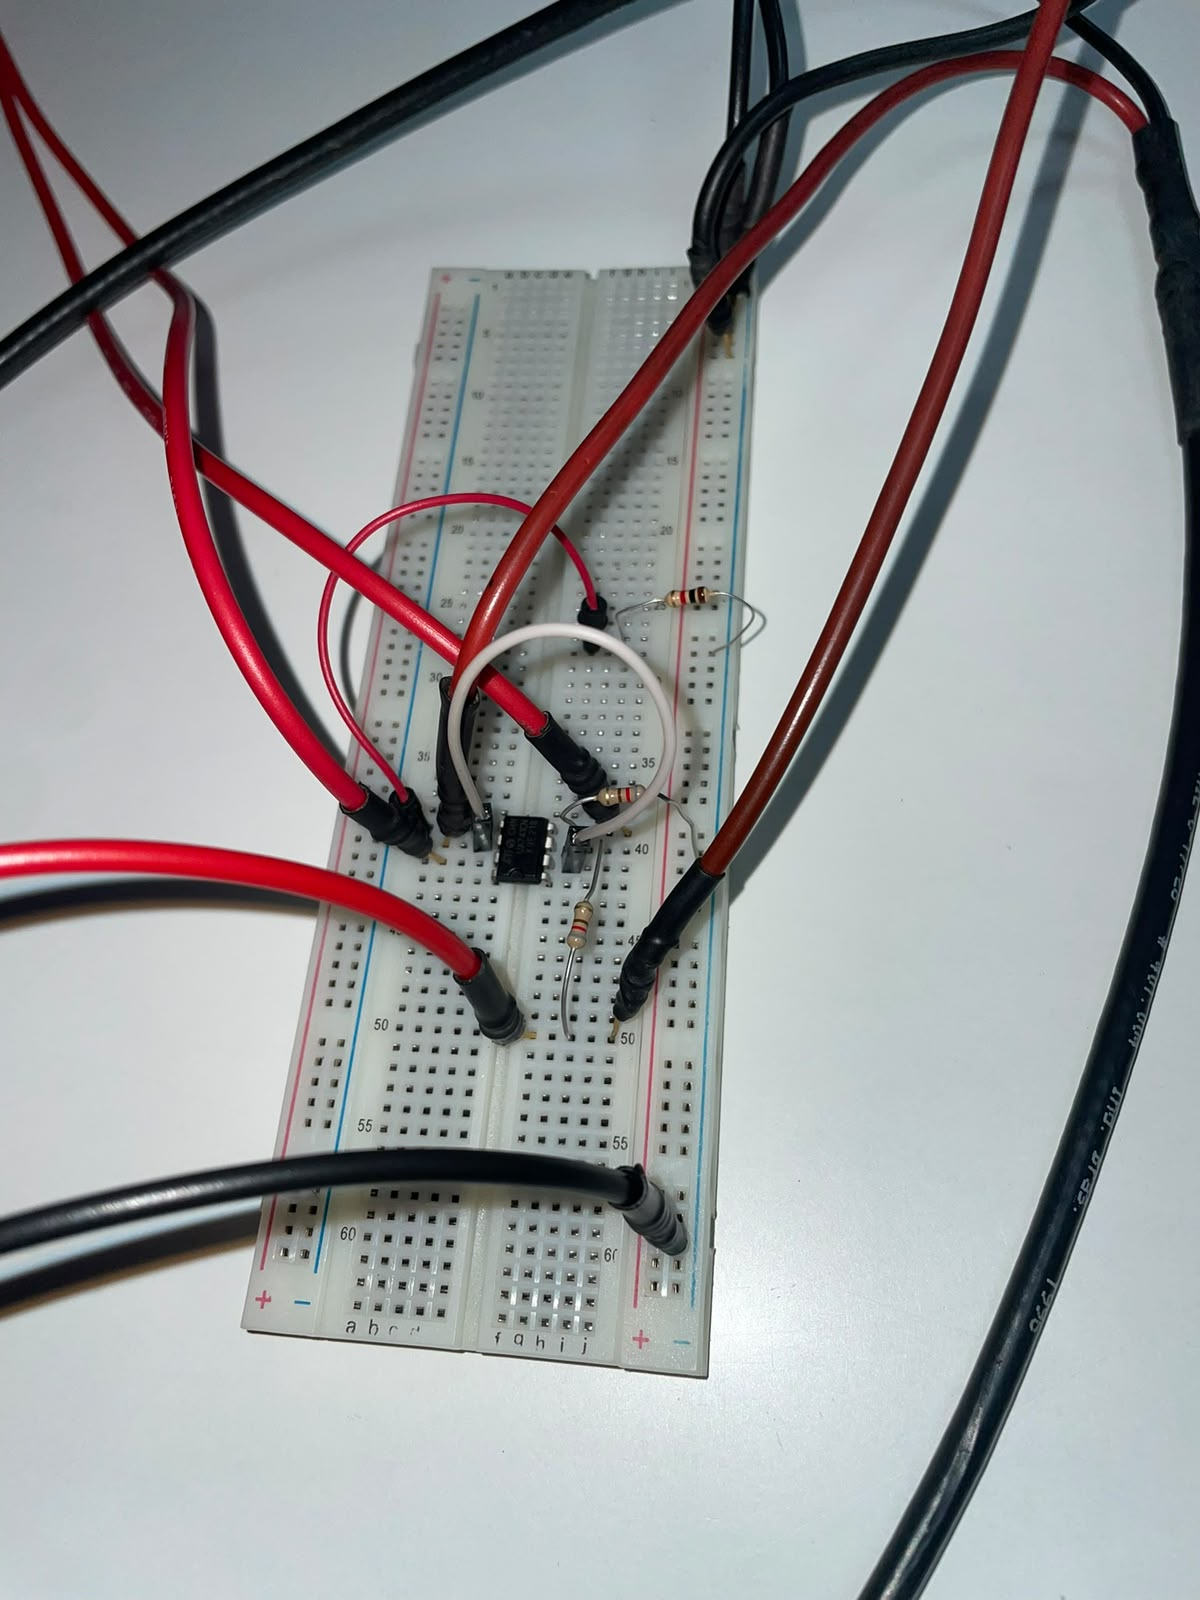
\includegraphics[width=0.55\linewidth]{circuito_3.3_4.png}
\caption{Seguidor de tensão montado na bancada (Equipe~1): divisor $R_1{=}R_2{=}820\,\Omega$
seguido do LM741 alimentando $R_L{=}1\,\text{k}\Omega$.}
\label{fig:bancada-seguidor}
\end{figure}

\subsection{Simulação da montagem}

Dos quatro circuitos, só o amplificador de diferença teve seus resistores medidos
individualmente nesta bancada. É essa medição que alimenta a Equação~\eqref{eq:acm} na
Seção~5.4, prevendo $A_d$ e o CMRR a partir só do descasamento real dos componentes — o
equivalente a uma simulação da montagem para esse circuito. Para o seguidor, o não inversor e
o somador, os resistores não foram pesados no multímetro nesta bancada, então a comparação da
Seção~6 usa a simulação de projeto diretamente contra a medição para esses três, sem essa etapa
intermediária.

\begin{nota}{Três comparações, três causas diferentes}
\textbf{Cálculo analítico contra simulação de projeto.} A conta está certa? Divergência aqui
vem da álgebra ou do esquemático.

\smallskip
\textbf{Simulação de projeto contra simulação da montagem.} Quanto custou a tolerância dos
componentes? A diferença aqui é a distância entre o valor nominal e o valor real da peça.

\smallskip
\textbf{Simulação da montagem contra medição.} O modelo descreve o circuito real? Diferença
aqui aponta algo que o modelo não representa — no caso do amplificador de diferença, por
exemplo, o CMRR do LM741 real usado no lugar do TL064 previsto.
\end{nota}

\section{Resultados}

\subsection{Projeto de cada integrante}

\textbf{Ana Luísa Reis Nascente.} Valores já deduzidos na Seção~3 (Teórico = especificação;
Adotado = simulado no LTspice com os resistores E12 escolhidos):

\begin{center}
\begin{tabular}{@{}llrrr@{}}
\toprule
\textbf{Item} & \textbf{Grandeza} & \textbf{Teórico} & \textbf{Simulado (adotado)} & \textbf{Desvio} \\
\midrule
1 & $V_{carga}$ (com carga) & $3{,}364$~V & $3{,}333$~V & $-0{,}9\%$ \\
2 & $G$ & $7{,}300$ & $7{,}305$ & $+0{,}07\%$ \\
3/4 & $k_1$ & $3{,}000$ & $2{,}973$ & $-0{,}90\%$ \\
3/4 & $k_2$ & $6{,}000$ & $5{,}946$ & $-0{,}90\%$ \\
5 & $A_d$ & $10{,}00$ & $10{,}00$ & $0{,}00\%$ \\
\bottomrule
\end{tabular}
\end{center}

\textbf{Gabriel de Sousa.} Especificação da Seção~4.1 contra os componentes efetivamente
simulados em cada \texttt{item\_N.asc}:

\begin{center}
\begin{tabular}{@{}llrrr@{}}
\toprule
\textbf{Item} & \textbf{Grandeza} & \textbf{Teórico} & \textbf{Simulado (adotado)} & \textbf{Desvio} \\
\midrule
1 & $R_{th}$ mínimo & $333{,}3\,\Omega$ & $776{,}5\,\Omega$ (folga) & — \\
1 & Queda (com carga direta) & $25{,}0\%$ (mínimo) & $43{,}7\%$ & acima do mínimo \\
2 & $G$ & $10{,}80$ & $10{,}50$ & $-2{,}8\%$ \\
3/4 & $k_1$ & $2{,}000$ & $2{,}000$ & $0{,}00\%$ \\
3/4 & $k_2$ & $6{,}000$ & $6{,}000$ & $0{,}00\%$ \\
5 & $A_d$ & $2{,}000$ & $8{,}000$ & $+300\%$ \\
\bottomrule
\end{tabular}
\end{center}

O item~5 de Gabriel destoa dos demais: a especificação da matrícula pede $A_d{=}2{,}0$
(pois $GH{=}00$ e $I{=}0$ zeram o termo da Equação de $A_d$), mas o esquemático simulado usa
$R_2/R_1=12\text{k}/1{,}5\text{k}=8{,}0$ — a mesma razão do somador (item\_3/4), o que sugere
reaproveitamento acidental dos valores de $R_f$ do somador ao montar o item\_5. Os demais
itens (1 a 4) fecham dentro do esperado para arredondamento em série E12 ou exatos.

\subsection{Seguidor de tensão}

Nesta bancada, o efeito de carregamento foi registrado com o seguidor já entre o divisor e a
carga: sem carga, a saída do seguidor tem $4{,}00\,\text{V}_{pp}$; com $R_L{=}1\,\text{k}
\Omega$ ligada, cai para $3{,}92\,\text{V}_{pp}$ — uma queda de apenas ${\approx}2\%$. O
divisor sozinho, sem o seguidor, não chegou a ser medido separadamente nesta bancada.

\textbf{Questão (impedância de entrada e saída).} A especificação de bancada prevê uma queda
de $29\%$ para o divisor alimentando a carga diretamente, contra a queda de ${\approx}2\%$
medida com o seguidor no meio. Como a carga é a mesma nos dois casos, a diferença só pode vir
do circuito que a alimenta: o divisor sozinho tem impedância de saída da mesma ordem da carga
(por isso a sente), enquanto o seguidor tem impedância de saída muito menor e por isso
praticamente não é afetado por ela. Do lado da entrada, o próprio mecanismo do curto virtual —
a saída do seguidor reproduz $v_i$ na entrada inversora sem que o AmpOp drene corrente do
divisor — garante que sua impedância de entrada seja muito maior que $R_2$.

\subsection{Amplificador não inversor}

\begin{center}
\begin{tabular}{@{}lrrrr@{}}
\toprule
\textbf{Grandeza} & \textbf{Projeto} & \textbf{Sim. montagem} & \textbf{Medido} & \textbf{Erro} \\
\midrule
Ganho $G_v$ & $2{,}00$ & & $2{,}00$ & $0\%$ \\
Ganho $G_v$ (AmpOp livre do TL064) & $2{,}00$ & & $2{,}02$ & $1{,}0\%$ \\
Saturação positiva & & & $+13{,}6\,\text{V}$ & \\
Saturação negativa & & & $-14{,}4\,\text{V}$ & \\
$V^+$ (pino 7) & $+15\,\text{V}$ & & $+14{,}997\,\text{V}$ & $-0{,}02\%$ \\
$V^-$ (pino 4) & $-15\,\text{V}$ & & $-14{,}139\,\text{V}$ & $-5{,}7\%$ \\
\bottomrule
\end{tabular}
\end{center}

\begin{figure}[htb]
\centering
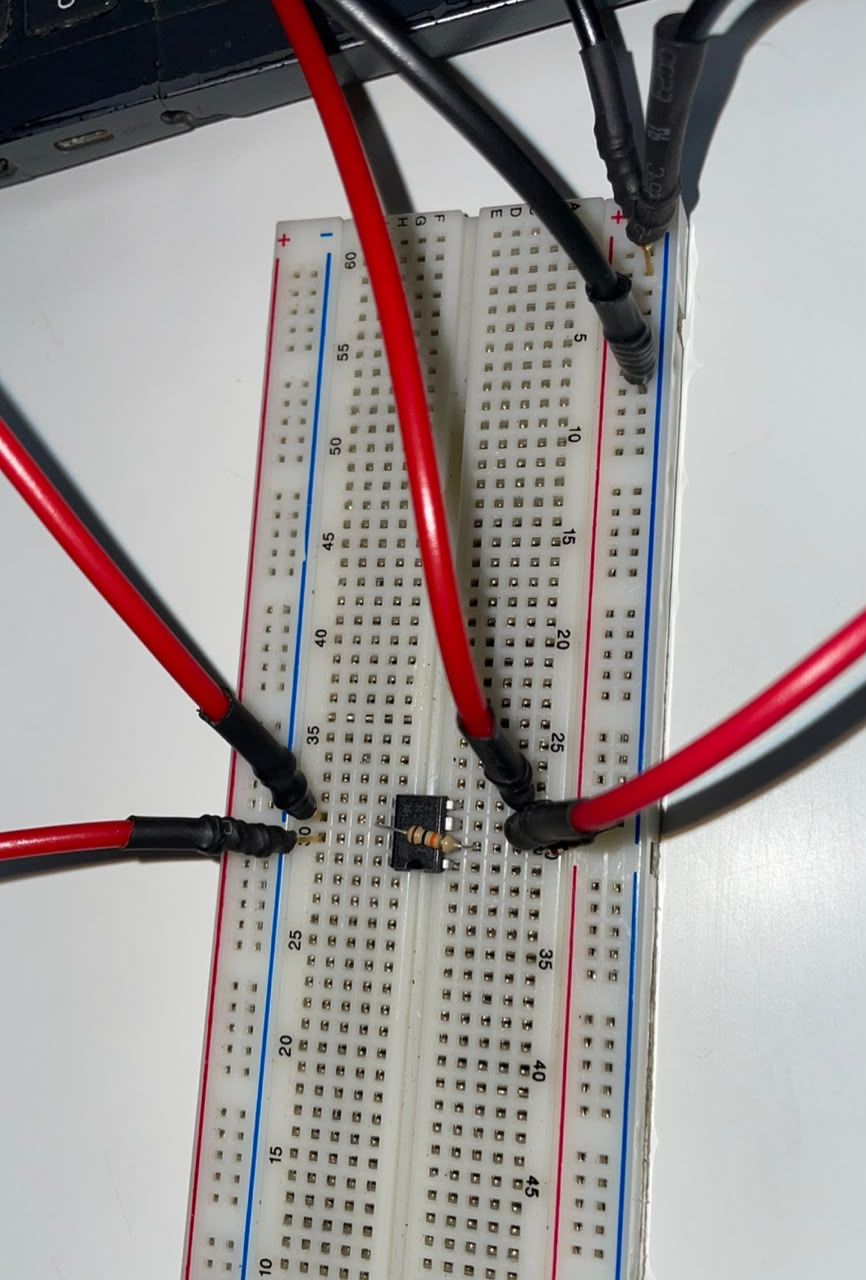
\includegraphics[width=0.32\linewidth]{circuito_3.4_1.png}\hfill
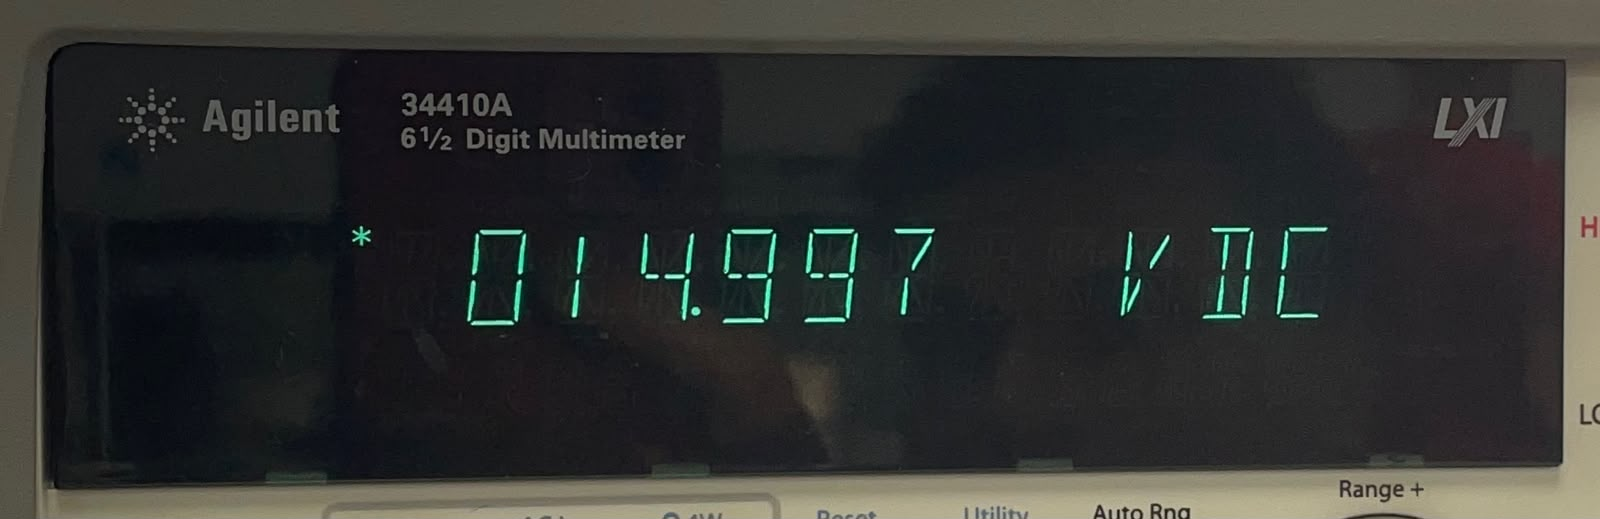
\includegraphics[width=0.32\linewidth]{multimetro_3.4_pino7.png}\hfill
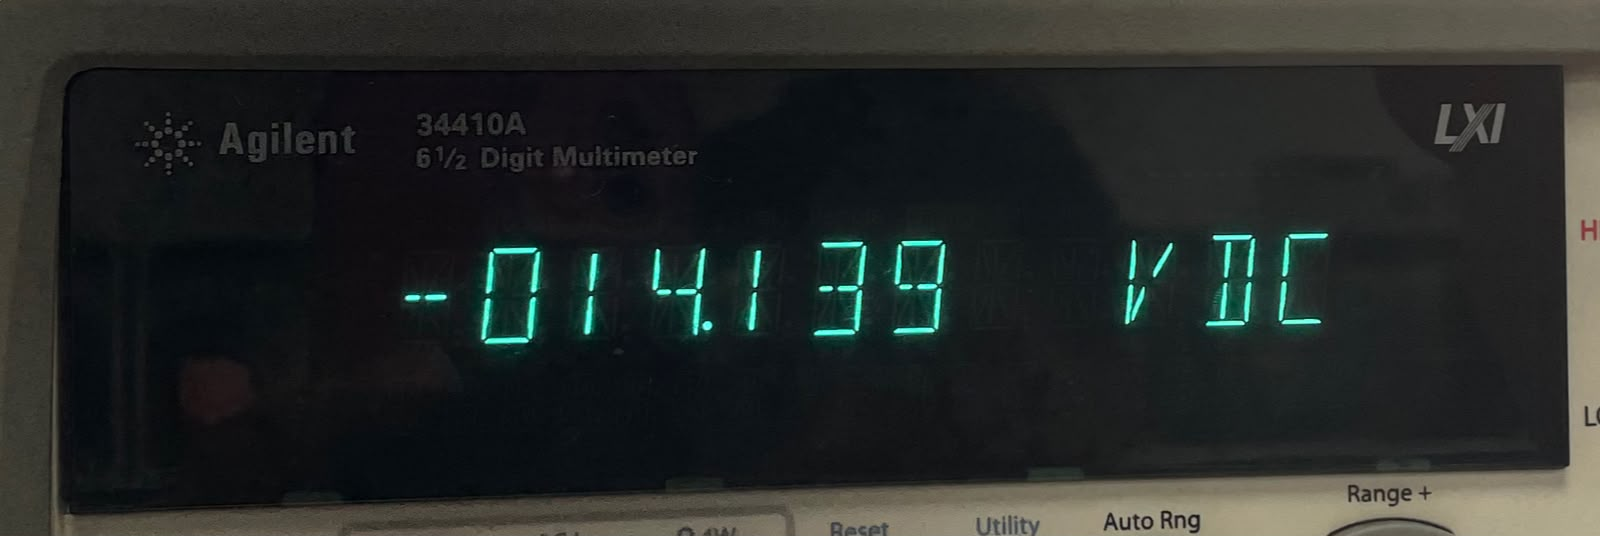
\includegraphics[width=0.32\linewidth]{multimetro_3.4_pino4.png}
\caption{Não inversor montado (LM741) e os multímetros nos pinos de alimentação: pino~7
($V^+{=}+14{,}997\,\text{V}$) e pino~4 ($V^-{=}-14{,}139\,\text{V}$).}
\label{fig:bancada-naoinversor}
\end{figure}

O pino 7 chega a $+14{,}997\,\text{V}$, praticamente sem queda em relação aos $+15\,\text{V}$
nominais da fonte ($-0{,}02\%$); o pino 4 chega a apenas $-14{,}139\,\text{V}$, uma queda de
$0{,}861\,\text{V}$ ($-5{,}7\%$) — bem maior que a do trilho positivo. Os dois sinais batem com
o que se espera fisicamente (nenhuma inversão de ponta), mas a assimetria entre os dois trilhos
não é explicada só pelo circuito: é provável que o fio ou o contato do trilho negativo na
protoboard tenha resistência de contato maior que o do positivo.

\textbf{Questão (o ganho depende do amplificador ou dos resistores?).} Trocando o LM741 por um
AmpOp livre do TL064, sem alterar $R_f$ nem $R_g$, o ganho medido passou de $2{,}00$ para
$2{,}02$ — praticamente o mesmo. Isso confirma que, sob realimentação negativa com ganho de
malha aberta muito maior que $G$, o ganho fechado depende só da razão $R_f/R_g$, não do AmpOp
específico.

\textbf{Questão (por que a saída não alcança a alimentação?).} O estágio de saída do AmpOp tem
sua própria queda de tensão interna, então a excursão máxima fica sempre um pouco abaixo do que
chega nos pinos de alimentação — mesmo com $+14{,}997\,\text{V}$ no pino 7, a saída só sobe até
$+13{,}6\,\text{V}$ (dropout de $1{,}4\,\text{V}$); com $-14{,}139\,\text{V}$ no pino 4, a saída
desce até $-14{,}4\,\text{V}$. Esse segundo número — saída mais negativa que o próprio pino de
alimentação medido — é fisicamente impossível para o mesmo instante de operação, o que indica
que a saturação e a leitura do pino 4 não foram registradas sob exatamente as mesmas condições
de carga da fonte (ex.: a fonte pode ter caído mais sob o sinal grande de saturação do que no
repouso da medida DC do pino). Fica como ressalva: o dropout do lado negativo, calculado aqui,
é uma estimativa de limite inferior.

\subsection{Somador inversor}

\begin{figure}[htb]
\centering
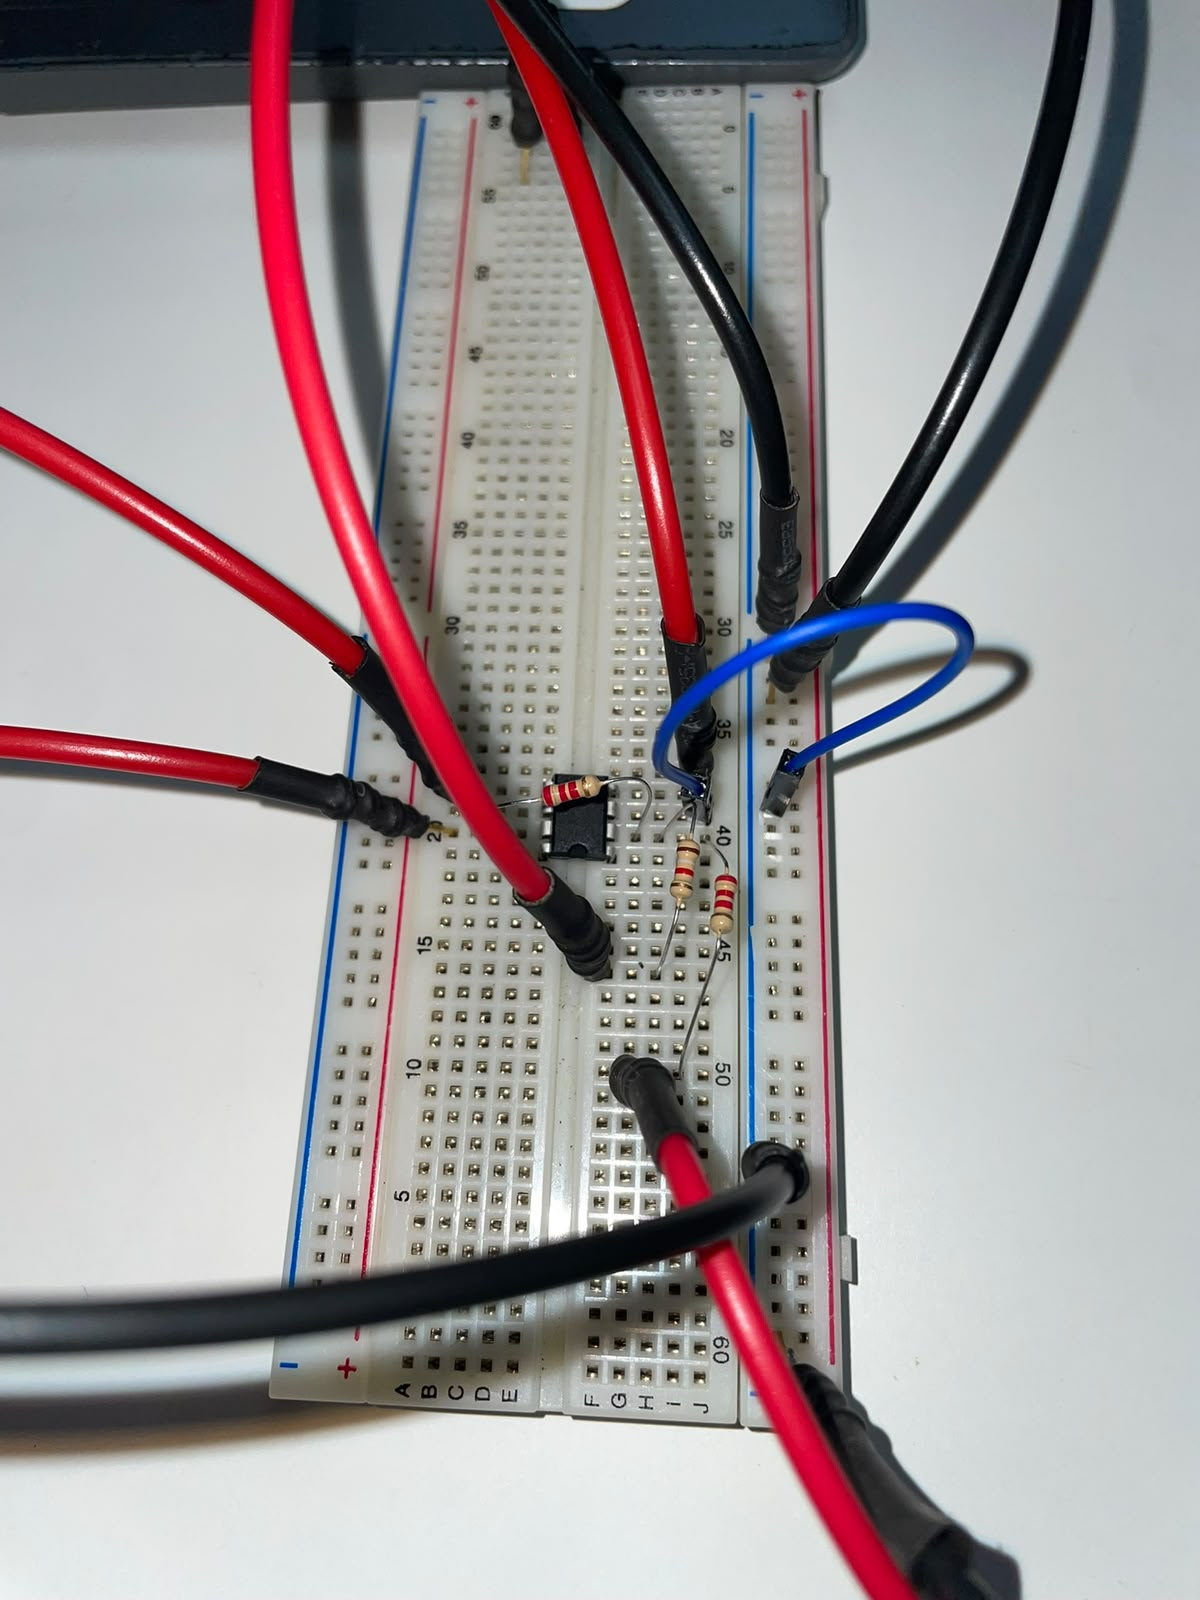
\includegraphics[width=0.5\linewidth]{circuito_3.5.png}
\caption{Somador inversor montado na bancada: LM741 com
$R_1{=}R_f{=}2{,}2\,\text{k}\Omega$ e $R_2{=}1{,}8\,\text{k}\Omega$.}
\label{fig:bancada-somador}
\end{figure}

Com os resistores efetivamente usados ($R_1{=}R_f{=}2{,}2\,\text{k}\Omega$,
$R_2{=}1{,}8\,\text{k}\Omega$), os pesos ficam $k_1{=}R_f/R_1{=}1{,}000$ e
$k_2{=}R_f/R_2{=}1{,}222$, praticamente iguais à especificação de bancada ($k_1{=}1{,}00$,
$k_2{=}1{,}22$). Com $V_1{=}4{,}0\,\text{V}$ e $V_2{=}-4{,}0\,\text{V}$, o projeto prevê
$V_o=-(k_1V_1+k_2V_2)=-(1{,}000\times4{,}0+1{,}222\times(-4{,}0))=+0{,}89\,\text{V}$.

\begin{center}
\begin{tabular}{@{}lrl@{}}
\toprule
\textbf{Grandeza} & \textbf{Projeto} & \textbf{Medido} \\
\midrule
$V_2$ (DC) & $-4{,}00\,\text{V}$ & $-4{,}00\,\text{V}$ \\
$V_1$ (DC, multímetro) & $+4{,}00\,\text{V}$ & $+3{,}87\,\text{V}$ \\
$V_1$ (osciloscópio) & constante & ondulação de $4{,}00\,\text{V}_{pp}$ em $666{,}7\,\text{Hz}$ \\
Saída & $+0{,}89\,\text{V}$ & centrada em ${\approx}4{,}92\,\text{V}$, $3{,}92\,\text{V}_{pp}$ \\
\bottomrule
\end{tabular}
\end{center}

O multímetro, que faz a média, lê $V_1{\approx}3{,}87\,\text{V}$ e $V_2{=}-4{,}00\,\text{V}$,
ambos perto do projetado. Mas o osciloscópio mostra que o nó de $V_1$ não está parado em DC —
há uma ondulação de $4{,}00\,\text{V}_{pp}$ em torno da média — e a saída herda essa ondulação,
ficando bem longe do $+0{,}89\,\text{V}$ constante esperado. Isso indica que $V_1$ não estava
de fato preso a uma fonte DC estável no instante da medida, provavelmente ligado à fonte de
sinal (gerador de função) em vez da fonte DC da bancada.

\textbf{Verificação e questão (curto virtual e isolamento entre entradas).} A tensão entre as
duas entradas do AmpOp ficou em $-0{,}004\,\text{mV}$, e a do nó somador em relação ao terra em
$-0{,}006\,\text{mV}$ — resíduos na casa de microvolts, consistentes com o modelo de curto
virtual. É esse terra virtual que responde à pergunta do roteiro sobre isolamento entre as
entradas: como o nó inversor fica preso a ${\approx}0\,\text{V}$ independentemente do que cada
entrada faça, cada resistor de entrada vê sempre o mesmo curto para o terra — nenhuma das duas
entradas enxerga a outra, e a corrente que cada uma injeta sai inteira pelo resistor de
realimentação, como previsto pela Equação~\eqref{eq:somador}.

\subsection{Amplificador de diferença}

\begin{figure}[htb]
\centering
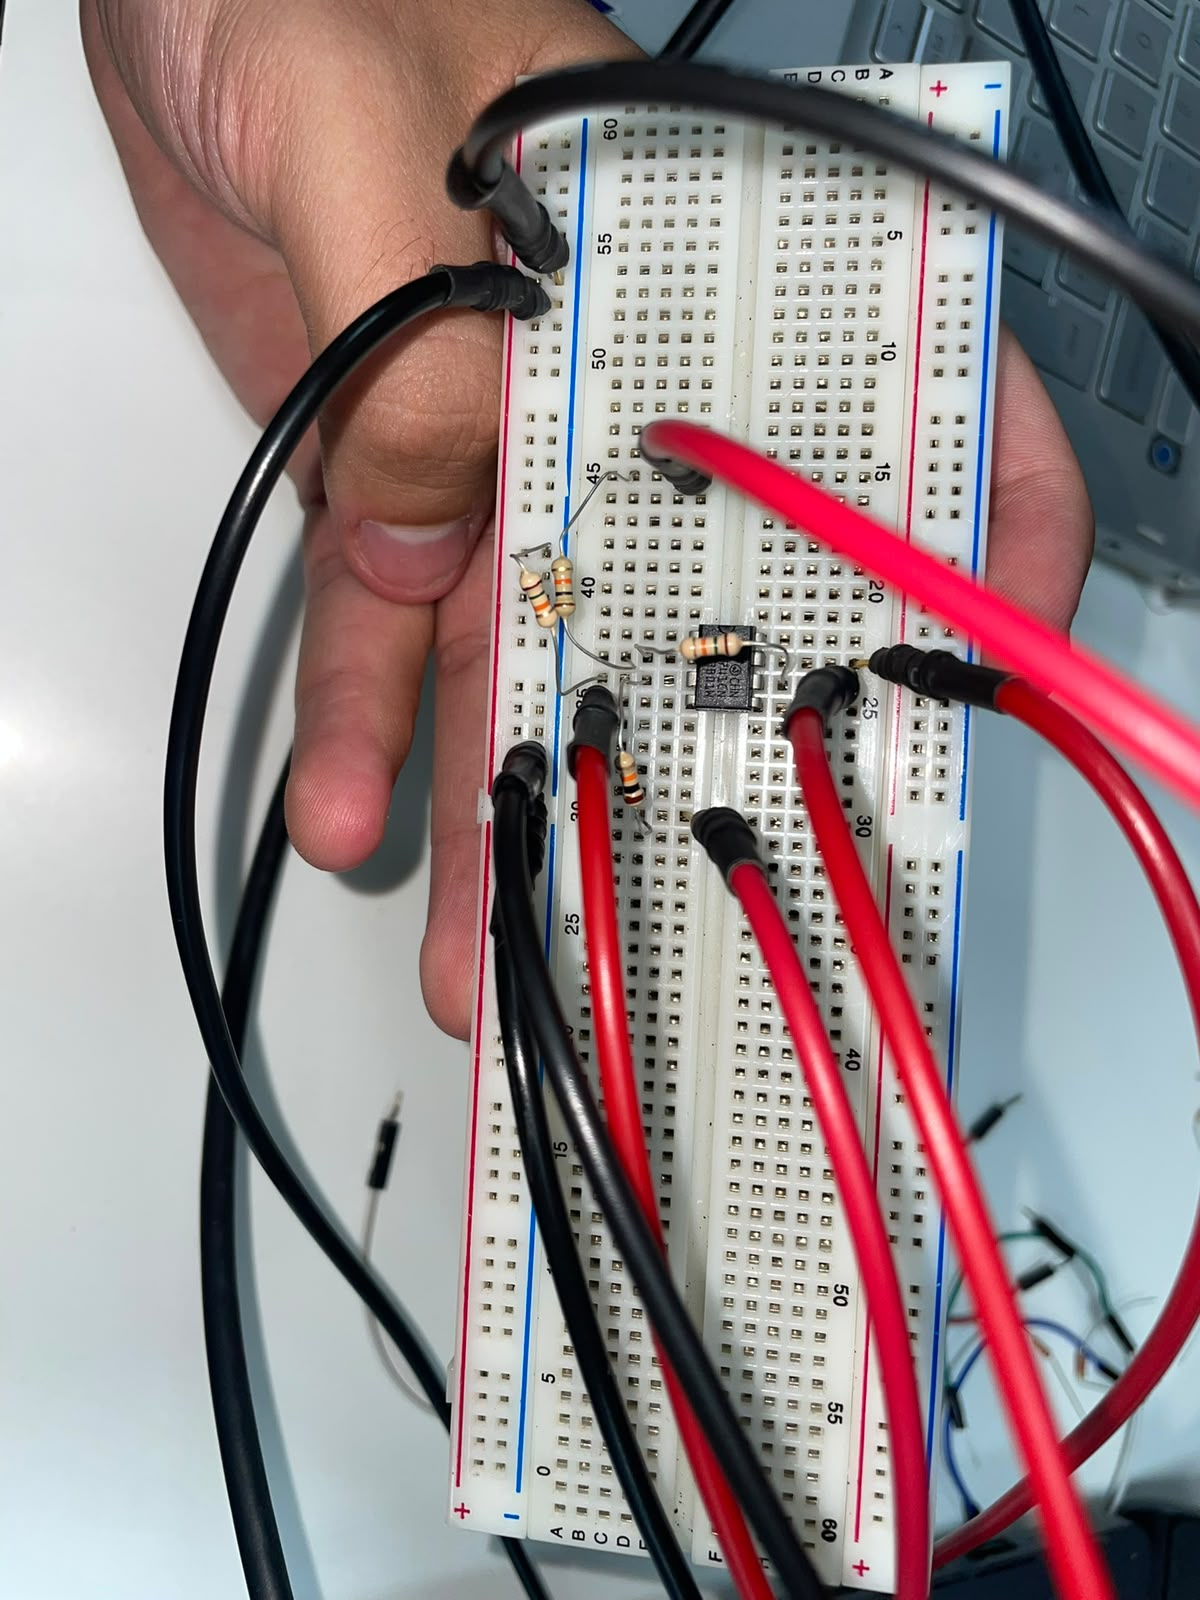
\includegraphics[width=0.42\linewidth]{circuito_3.6.png}
\caption{Amplificador de diferença montado na bancada, com o LM741 no lugar do TL064
especificado.}
\label{fig:bancada-diferenca}
\end{figure}

\begin{center}
\begin{tabular}{@{}lrrrr@{}}
\toprule
\textbf{Grandeza} & \textbf{Projeto} & \textbf{Sim. montagem} & \textbf{Medido} & \textbf{Erro} \\
\midrule
$A_d$ & $1{,}50$ & & $1{,}45$ & $-3{,}3\%$ \\
$A_{cm}$ & $0$ (ideal) & & $0{,}0228$ & \\
CMRR & — & & $36{,}1\,\text{dB}$ & \\
\bottomrule
\end{tabular}
\end{center}

\begin{figure}[htb]
\centering
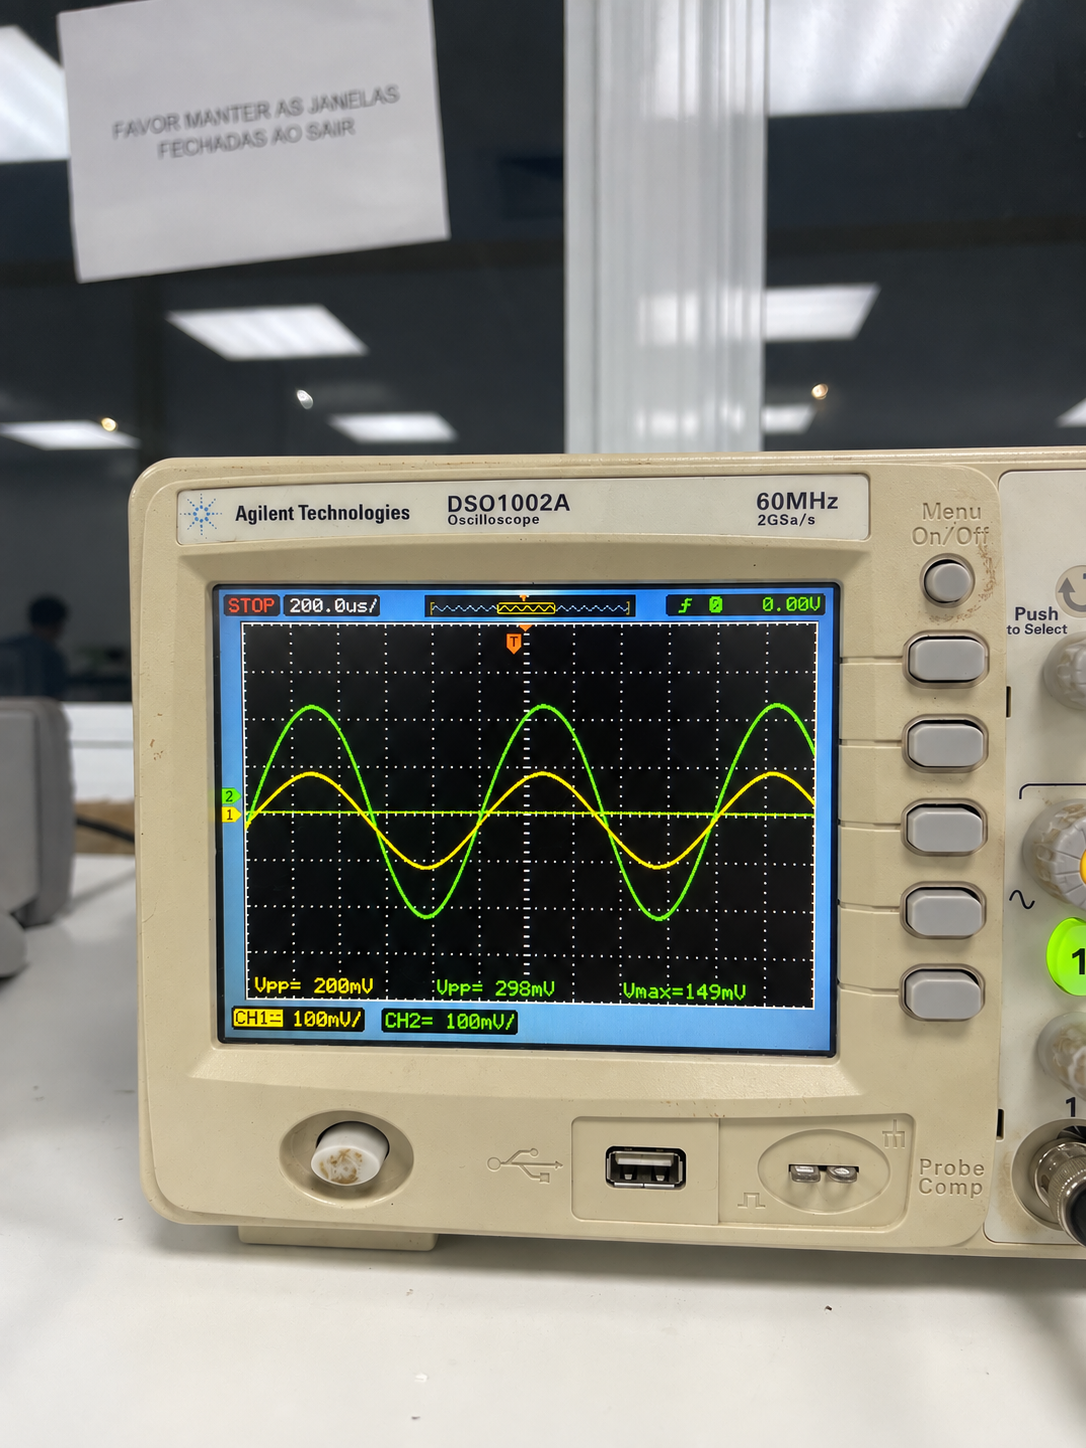
\includegraphics[width=0.47\linewidth]{grafico_3.6_diferencial.png}\hfill
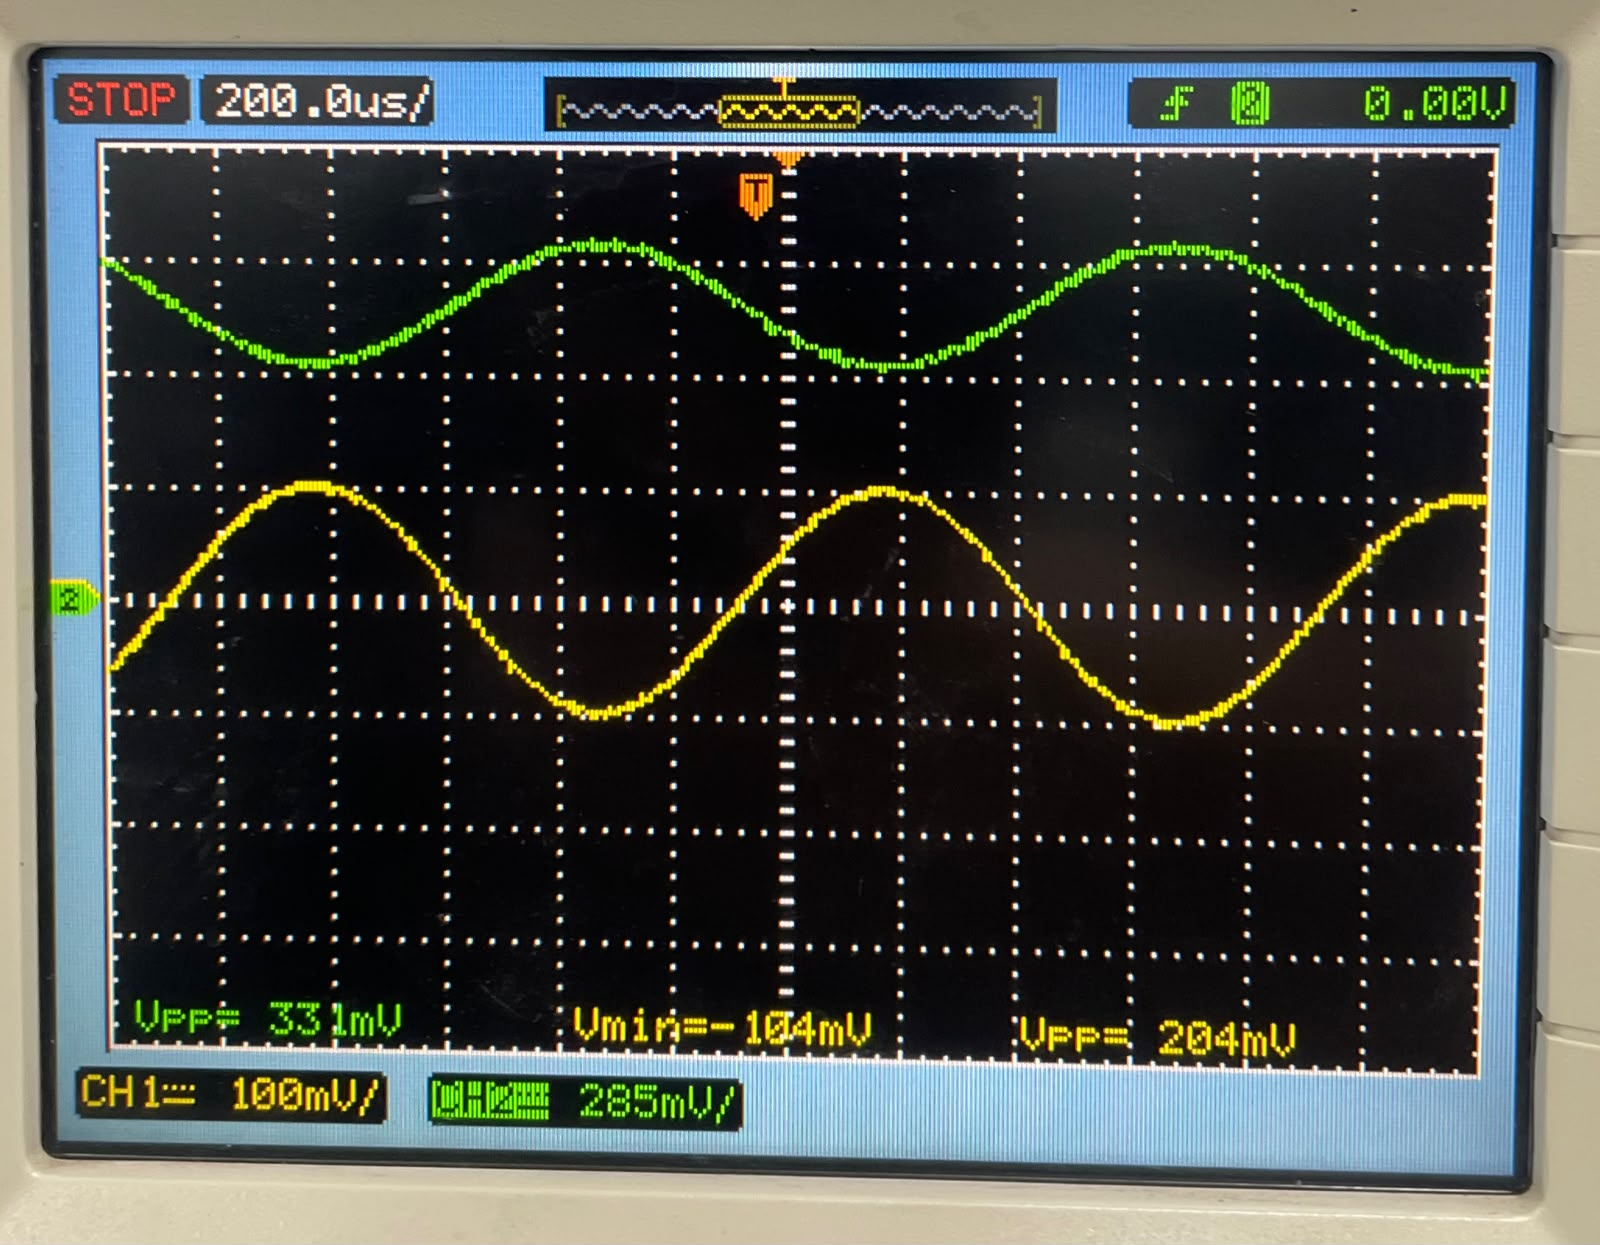
\includegraphics[width=0.47\linewidth]{grafico_3.6_modocomum.png}
\caption{Osciloscópio no ensaio diferencial ($V_{pp,\text{entrada}}{=}200\,\text{mV}$,
$V_{pp,\text{saída}}{=}298\,\text{mV}$, à esquerda) e no ensaio de modo comum (à direita), usados
para calcular $A_d$, $A_{cm}$ e o CMRR da tabela acima.}
\label{fig:bancada-diferenca-graficos}
\end{figure}

Com os quatro resistores medidos ($R_1{=}9{,}97\,\text{k}\Omega$,
$R_2{=}14{,}95\,\text{k}\Omega$, $R_3{=}10{,}05\,\text{k}\Omega$,
$R_4{=}15{,}01\,\text{k}\Omega$), a Equação~\eqref{eq:acm} prevê, só a partir do descasamento
dos resistores: $A_d{=}1{,}4995$, $A_{cm}{=}0{,}0024$, $\text{CMRR}{=}56{,}0\,\text{dB}$.

\textbf{Verificação / Questão (de onde vem o ganho de modo comum medido?).} O CMRR previsto
só pelo descasamento dos resistores ($56{,}0\,\text{dB}$) é bem melhor que o CMRR realmente
medido ($36{,}1\,\text{dB}$) — uma diferença de $20\,\text{dB}$, ou seja, o $A_{cm}$ real é
cerca de $10\times$ maior que o previsto só pelos resistores. A causa não pode ser o
descasamento dos resistores, já que ele prevê rejeição melhor do que a obtida: o limite real
vem do próprio LM741, um AmpOp de uso geral sem otimização para rejeição de modo comum — e
usado aqui no lugar do TL064 especificado, o que provavelmente piora ainda mais essa
rejeição.

\section{Discussão}

A Seção~4.3 propôs três comparações independentes — cálculo contra simulação de projeto,
simulação de projeto contra simulação da montagem, e simulação da montagem contra medição —
cada uma isolando uma causa de divergência diferente. A simulação da montagem (com os
resistores medidos no lugar dos nominais) não foi refeita para seguidor, não inversor e
somador por falta da medição desses resistores na bancada, então, para esses três circuitos,
a análise abaixo colapsa a segunda e a terceira comparação numa só: projeto contra medição.

\textbf{Seguidor de tensão.} O cálculo bate com o esperado por construção — a Equação~\eqref{eq:queda}
não deixa margem para erro de álgebra, só para escolha de $R_{th}$. A medição confirma o efeito
qualitativo previsto: queda de ${\approx}29\%$ especificada para o divisor sem seguidor contra
${\approx}2\%$ medida com o seguidor entre o divisor e a carga (Seção~5.2), o que já demonstra
a alta impedância de entrada e a baixa impedância de saída do AmpOp. Como os resistores desse
circuito não foram medidos individualmente nesta bancada (Seção~4.3), a comparação aqui é
direta entre projeto e medição, sem isolar separadamente o efeito da tolerância dos
componentes.

\textbf{Amplificador não inversor.} Cálculo e simulação de projeto batem por construção
($R_f/R_g$ escolhido para casar $G_v{=}2{,}00$ exatamente, já que $10\,\text{k}\Omega/10\,
\text{k}\Omega$ é um valor E12 direto, sem arredondamento). A medição reproduz esse ganho
exatamente ($G_v{=}2{,}00$, erro $0\%$) e se mantém praticamente igual ao trocar o LM741 pelo
TL064 ($G_v{=}2{,}02$), confirmando que o ganho fechado depende só da razão $R_f/R_g$. A única
divergência real entre montagem e medição apareceu na alimentação: o pino~7 chega bem perto do
nominal ($+14{,}997\,\text{V}$, $-0{,}02\%$), mas o pino~4 fica $0{,}861\,\text{V}$ abaixo do
nominal ($-5{,}7\%$) — mais provavelmente contato ou fio com resistência maior nesse trilho da
protoboard do que qualquer efeito do circuito projetado.

\textbf{Somador inversor.} O cálculo com os resistores realmente usados prevê
$V_o{=}+0{,}89\,\text{V}$ (Seção~5.3), e a verificação de curto virtual bate com o modelo
(resíduos na casa de microvolts). Mas a medição não reproduz esse valor: o multímetro (que
faz a média) lê $V_1{\approx}3{,}87\,\text{V}$, perto do projetado, porém o osciloscópio mostra
esse mesmo nó com uma ondulação de $4{,}00\,\text{V}_{pp}$ que deveria ser DC, e a saída herda
essa ondulação. Essa divergência não é sobre tolerância de resistor nem sobre o modelo do
AmpOp — é uma falha na própria fonte de $V_1$ na bancada, provavelmente ligada ao gerador de
função em vez da fonte DC, e por isso cai fora das três causas do quadro da Seção~4.3: é um
problema de montagem, não de projeto ou de modelo.

\textbf{Amplificador de diferença.} Com os quatro resistores medidos, o cálculo por
\eqref{eq:acm} prevê $A_d{=}1{,}4995$ e $\text{CMRR}{=}56{,}0\,\text{dB}$ — ou seja, o
descasamento dos resistores por si só permitiria uma rejeição de modo comum boa. A medição,
porém, deu $\text{CMRR}{=}36{,}1\,\text{dB}$, $20\,\text{dB}$ pior. Como o cálculo já usa os
valores medidos dos resistores, essa diferença não pode vir da tolerância dos componentes —
sobra o próprio AmpOp: o LM741 é um dispositivo de uso geral, sem otimização para rejeição de
modo comum, usado aqui no lugar do TL064 especificado por falta do encapsulamento na bancada.
É o único dos quatro circuitos em que a segunda causa do quadro (modelo não representa o
circuito real) domina claramente sobre a primeira (tolerância dos componentes).

\section{Conclusão}

Os quatro blocos de realimentação negativa se comportaram como a teoria prevê sempre que a
bancada permitiu uma comparação limpa. O seguidor de tensão isolou a carga do divisor,
derrubando a queda de carregamento de ${\approx}29\%$ para ${\approx}2\%$; o não inversor
manteve o ganho fechado em $G_v{=}2{,}00$ trocando o AmpOp (LM741 por TL064), confirmando que o
ganho depende só da razão $R_f/R_g$; e o cálculo do amplificador de diferença com os resistores
medidos previu corretamente que a tolerância dos componentes não seria o fator limitante ali.

Os dois problemas encontrados são de naturezas distintas. O CMRR do amplificador de diferença
($36{,}1\,\text{dB}$ medido contra $56{,}0\,\text{dB}$ previsto só pelos resistores) é uma
limitação real e explicável: o LM741 usado no lugar do TL064 não foi projetado para rejeição de
modo comum, e a substituição forçada pela falta do componente na bancada custou exatamente essa
margem. Já a ondulação de $4\,\text{V}_{pp}$ medida na entrada $V_1$ do somador, que deveria ser
uma tensão DC constante, é uma falha de montagem (provavelmente a fonte de sinal ligada no
lugar da fonte DC) que este relatório não chega a resolver — mas que já está isolada das outras
três causas de divergência do quadro da Seção~4.3, já que a verificação de curto virtual do
somador se manteve consistente com o modelo em todo o resto do circuito.

Do ponto de vista de projeto, o exercício de aproximar razões de resistores pela série E12
mostrou que o erro de arredondamento é pequeno e controlável quando se permite combinar dois
resistores em série (erro de $0{,}07\%$ a $0{,}9\%$ nos itens deste relatório) — bem menor do
que os efeitos que dominaram a montagem real: contato/fio de resistência maior num trilho de
alimentação, substituição de componente por indisponibilidade, e uma fonte de sinal que não
entregou o DC esperado. Esses três são exatamente o tipo de imperfeição que só aparece na
bancada, não na simulação — e é por isso que as duas etapas, projeto simulado e medição real,
são necessárias e se complementam.

\section{Referências}

\begin{referencias}
\item SEDRA, A.~S.; SMITH, K.~C. \emph{Microeletrônica}. 5.~ed. São Paulo: Pearson
      Prentice Hall, 2007.
\item BOYLESTAD, R.~L.; NASHELSKY, L. \emph{Dispositivos Eletrônicos e Teoria de
      Circuitos}. 11.~ed. São Paulo: Pearson Education do Brasil, 2013.
\item Texas Instruments. \emph{LM741 Operational Amplifier}, datasheet.
\item Texas Instruments. \emph{TL064 Low-Power JFET-Input Operational Amplifiers}, datasheet.
\end{referencias}

\end{document}
